\section{Descripcion de los Experimentos}
 \subsection{Experimento 1: Selección de Herramienta para la toma de Métricas de Consumo}\label{exp1-selecttool}
En esta primera fase de experimentación se han llevado a cabo una comparativa entre las diferentes herramientas disponibles para la toma de métricas de consumo sobre cargas de trabajo desplegadas en contenedores. Estas cargas de trabajo están basadas en la codificación de video y se llevarán a cabo empleando la herramienta \textbf{ffmpeg}.

Se ha utilizado un unico video compuesto por los chunks \textbf{18 a 43} del video \textbf{Skateboarding\_CableLabs}, debido a que el objetivo principal es determinar qué herramienta es capaz de tomar el conjunto de métricas de consumo más precisas.

El video resultante de la union de los chuncks, consta de una duración de 50 segundos con un CRF 0 a una resolución 4K(3840 x 2160) y con un bitrate de 1012693 kbps (1012,693 Mbps). Pese a que no es un video con una gran duración, tiene una gran calidad con 0 pérdida y un bitrate muy elevado, proporcionando sufiente carga de trabajo al codificador. Permitiendo extraer suficientes métricas  en un tiempo prolongado del proceso de codificación mediante CPU y GPU, ya que, por lo general, los códecs que utilizan la GPU para llevar a cabo la codificación son notablemente más rápidos que los codificadores que utilizan codificación únicamente sobre CPU.
\begin{lstlisting}[language=sh,label={code:exp1-ffmpeg-encoding},caption={Orden de codificación para codificadores CPU y codificadores GPU}]
#Codificación empleando CPU
docker exec ffmpeg-container ffmpeg -y -i /config/SkLab_3840x2160_crf0.mp4 -c:v [ libx264 | libx265 ] -b:v 4M -vf scale=1280:720 -c:a copy /config/output.mp4

 # Codificación empleando CPU+GPU
 docker exec ffmpeg-container ffmpeg -y -i /config/SkLab_3840x2160_crf0.mp4 -c:v [ h264_nvenc | hevc_nvenc ] -b:v 4M -vf scale=1280:720 -c:a copy /config/output.mp4
\end{lstlisting}


\subsubsection{Desarrollo de los experimentos de la primera fase}

 En total se han definido cuatro escenarios experimentales, cuyo objetivo es evaluar la capacidad de cada herramienta para recopilar métricas de consumo energético, así como el nivel de granularidad de la información obtenida. Para la ejecución de estos experimentos se ha desarrollado un conjunto de scripts en Bash, encargados de automatizar tanto el despliegue de las pruebas como la recopilación de las métricas generadas por cada herramienta. Cada escenario se ejecutará un total de diez veces y, entre conjunto de iteraciones consecutivas, se establecerá un intervalo mínimo de dos minutos. Este intervalo tiene como objetivo reducir la influencia que el estado térmico del sistema tras las ejecuciones anteriores pueda ejercer sobre las mediciones, así como minimizar las variaciones inherentes a la ejecución de las cargas de trabajo. De este modo, se pretende obtener resultados más representativos y consistentes.
 
 Los scripts empleados para realizar las pruebas con Kepler \ref{exp1:kepler-script-probes} y Scaphandre \ref{exp1:scp-script-probes} comparten una estructura común, adaptando únicamente el proceso de inicialización y la recopilación de métricas a las particularidades de cada herramienta. En ambos casos es necesario especificar la ruta del vídeo que será codificado, el nombre del contenedor encargado de ejecutar el proceso de codificación y el directorio en el que se almacenarán las métricas obtenidas.
 
 Por otra parte, los scripts desarrollados para la herramienta Container Energy Monitoring \ref{exp1:monitor-script-probes-1container} y \ref{exp1:monitor-script-probes-2containers} requieren una configuración ligeramente más detallada. Además de indicar el contenedor que ejecutará la codificación y el directorio de salida de los resultados, es necesario definir el nombre del experimento, el número de iteraciones que se realizarán y el nombre de los archivos en los que se almacenarán las métricas recopiladas durante cada ejecución.
 
 Cabe destacar que, en el caso de Container Energy Meter, se han empleado dos scripts con el fin de evitar perder más tiempo y poder proseguir con la fase experimental 2, y poder cumplir con los plazos de entrega. Ambos scripts son prácticamente el mismo, a diferencia de \ref{exp1:monitor-script-probes-2containers} el cual lleva a cabo las acciones del script \ref{exp1:monitor-script-probes-1container} dos veces, almacenando los datos resultantes de la recolección en archivos diferenciados.


\subsection{Post-procesamiendo de las Métricas de Consumo Energético}
 Una vez finalizada la fase de experimentación, el procesamiento de los datos obtenidos en cada iteración se llevará a cabo mediante un nuevo conjunto de scripts desarrollados en Bash. Estos scripts se encargan de procesar las métricas recopiladas en cada ejecución, calcular el valor medio para cada escenario experimental y almacenar los resultados en un archivo CSV.
 
 En el caso de Kepler \ref{exp1:kepler-data-procesor} y Scaphandre \ref{exp1:scp-data-procesor}, el archivo CSV se genera en el mismo directorio donde se encuentran almacenados los datos de cada iteración. Por el contrario, la herramienta Container Energy Monitoring almacena el archivo resultante en un directorio denominado \texttt{data}. En todos los casos es necesario indicar la ruta donde se encuentran los datos que se desean procesar, así como el nombre del archivo CSV de salida.
 
 Aunque los archivos CSV generados por cada herramienta presentan una nomenclatura diferente, todos ellos contienen información equivalente relativa a las métricas de consumo energético recopiladas durante la experimentación. En las siguientes figuras se muestra un ejemplo de la cabecera generada por cada herramienta:

 \begin{figure}[h!]
      \centering
 	
\includegraphics[width=\linewidth]{figs/exp1_kepler_csv_header.png}  
 	\caption{Header CSV del archivo de datos procesados de Kepler}  
 	\label{fig:exp1-kepeler-csv_header}
 \end{figure}
 
 \begin{figure}[h!]
      \centering
 	
\includegraphics[width=\linewidth]{figs/exp1_scp_csv_header.png}  
 	\caption{Header CSV del archivo de datos procesados de Scaphandre}  
 	\label{fig:exp1-scp-csv_header}
 \end{figure}
 
 \begin{figure}[h!]
 \centering
 	
\includegraphics[width=\linewidth]{figs/exp1_monitor_csv_header.png}  
 	\caption{Header CSV del archivo de datos procesados de Container Energy Monitoring}  
 	\label{fig:exp1-monitor-csv_header}
 \end{figure}

Finalmente, para generar las tablas y gráficas comparativas entre las distintas herramientas en cada escenario experimental, se ha desarrollado un script en Python \ref{exp1:python-bar-grafics}. Este script procesa los archivos CSV generados por cada herramienta, calcula las métricas agregadas necesarias para el análisis comparativo y almacena los resultados en un nuevo archivo CSV. Dicho archivo constituye la entrada para la generación de las gráficas de barras histográficas y tablas comparativas que se presentan en el capítulo de resultados. 

A continuacion se detalla una lista de los posibles valores y su representación en la siguiente lista:
\begin{itemize} 
 \item \texttt{em\_total\_energy}: Energia total del sistema calculada en base añ consumo energetico de los grupos de comonentes $PKG+DRAM$ de RAPL estimada por Global Energy Meter. 
 \item \texttt{node\_total\_joules}: Energia total del sistema estimada por la herramient.
 \item \texttt{process$N$\_energy\_joules}: Energia total consumida por el proceso de transcodificacion $N$ estimado por la herramineta y ejecutado sobre el contenedor con \textit{FFMPEG}.  
 \item \texttt{gpu\_node\_jouls}: Energia consumida por la GPU durante el proceso de codificación estimado por la herramienta.
 \end{itemize}

\subsection{Analisis de resultante la sección Experimento 1}

\subsubsection{Escenario 1: Transcodificacion empleando un contenedor unicamente con CPU}
 En el siguiente escenario, se ha llevado a cabo la transcodificación de video sobre un contenedor utilizando un codificador basado CPU(\textit{x264} o \textit{x265}), cuyos resultados pueden apreciarse en la siguiente grafica de histogramas \ref{fig:exp1-es2-resultados}. 

 En relación a las métricas de consumo del nodo respecto a la metrics recolectadas por Global Energy Meter, se observa que la herramieta con menor discrepancia es \textbf{Global Energy Container}, con una tasa de error del \textbf{$0,3113\%$}. Seguido por \textbf{Scaphandre} con un \textbf{$3,4955\%$} y Kepler con un \textbf{$4,6850\%$}. 
 
 Estos resultado muestran como la capacidad para tomar métricas de consumo de un unico proceso ejecutado sobre un contenedor tiene mayor precision que \textit{Kepler} y a \textit{Scaphandre}.

 \begin{figure}[h!]
    \centering
    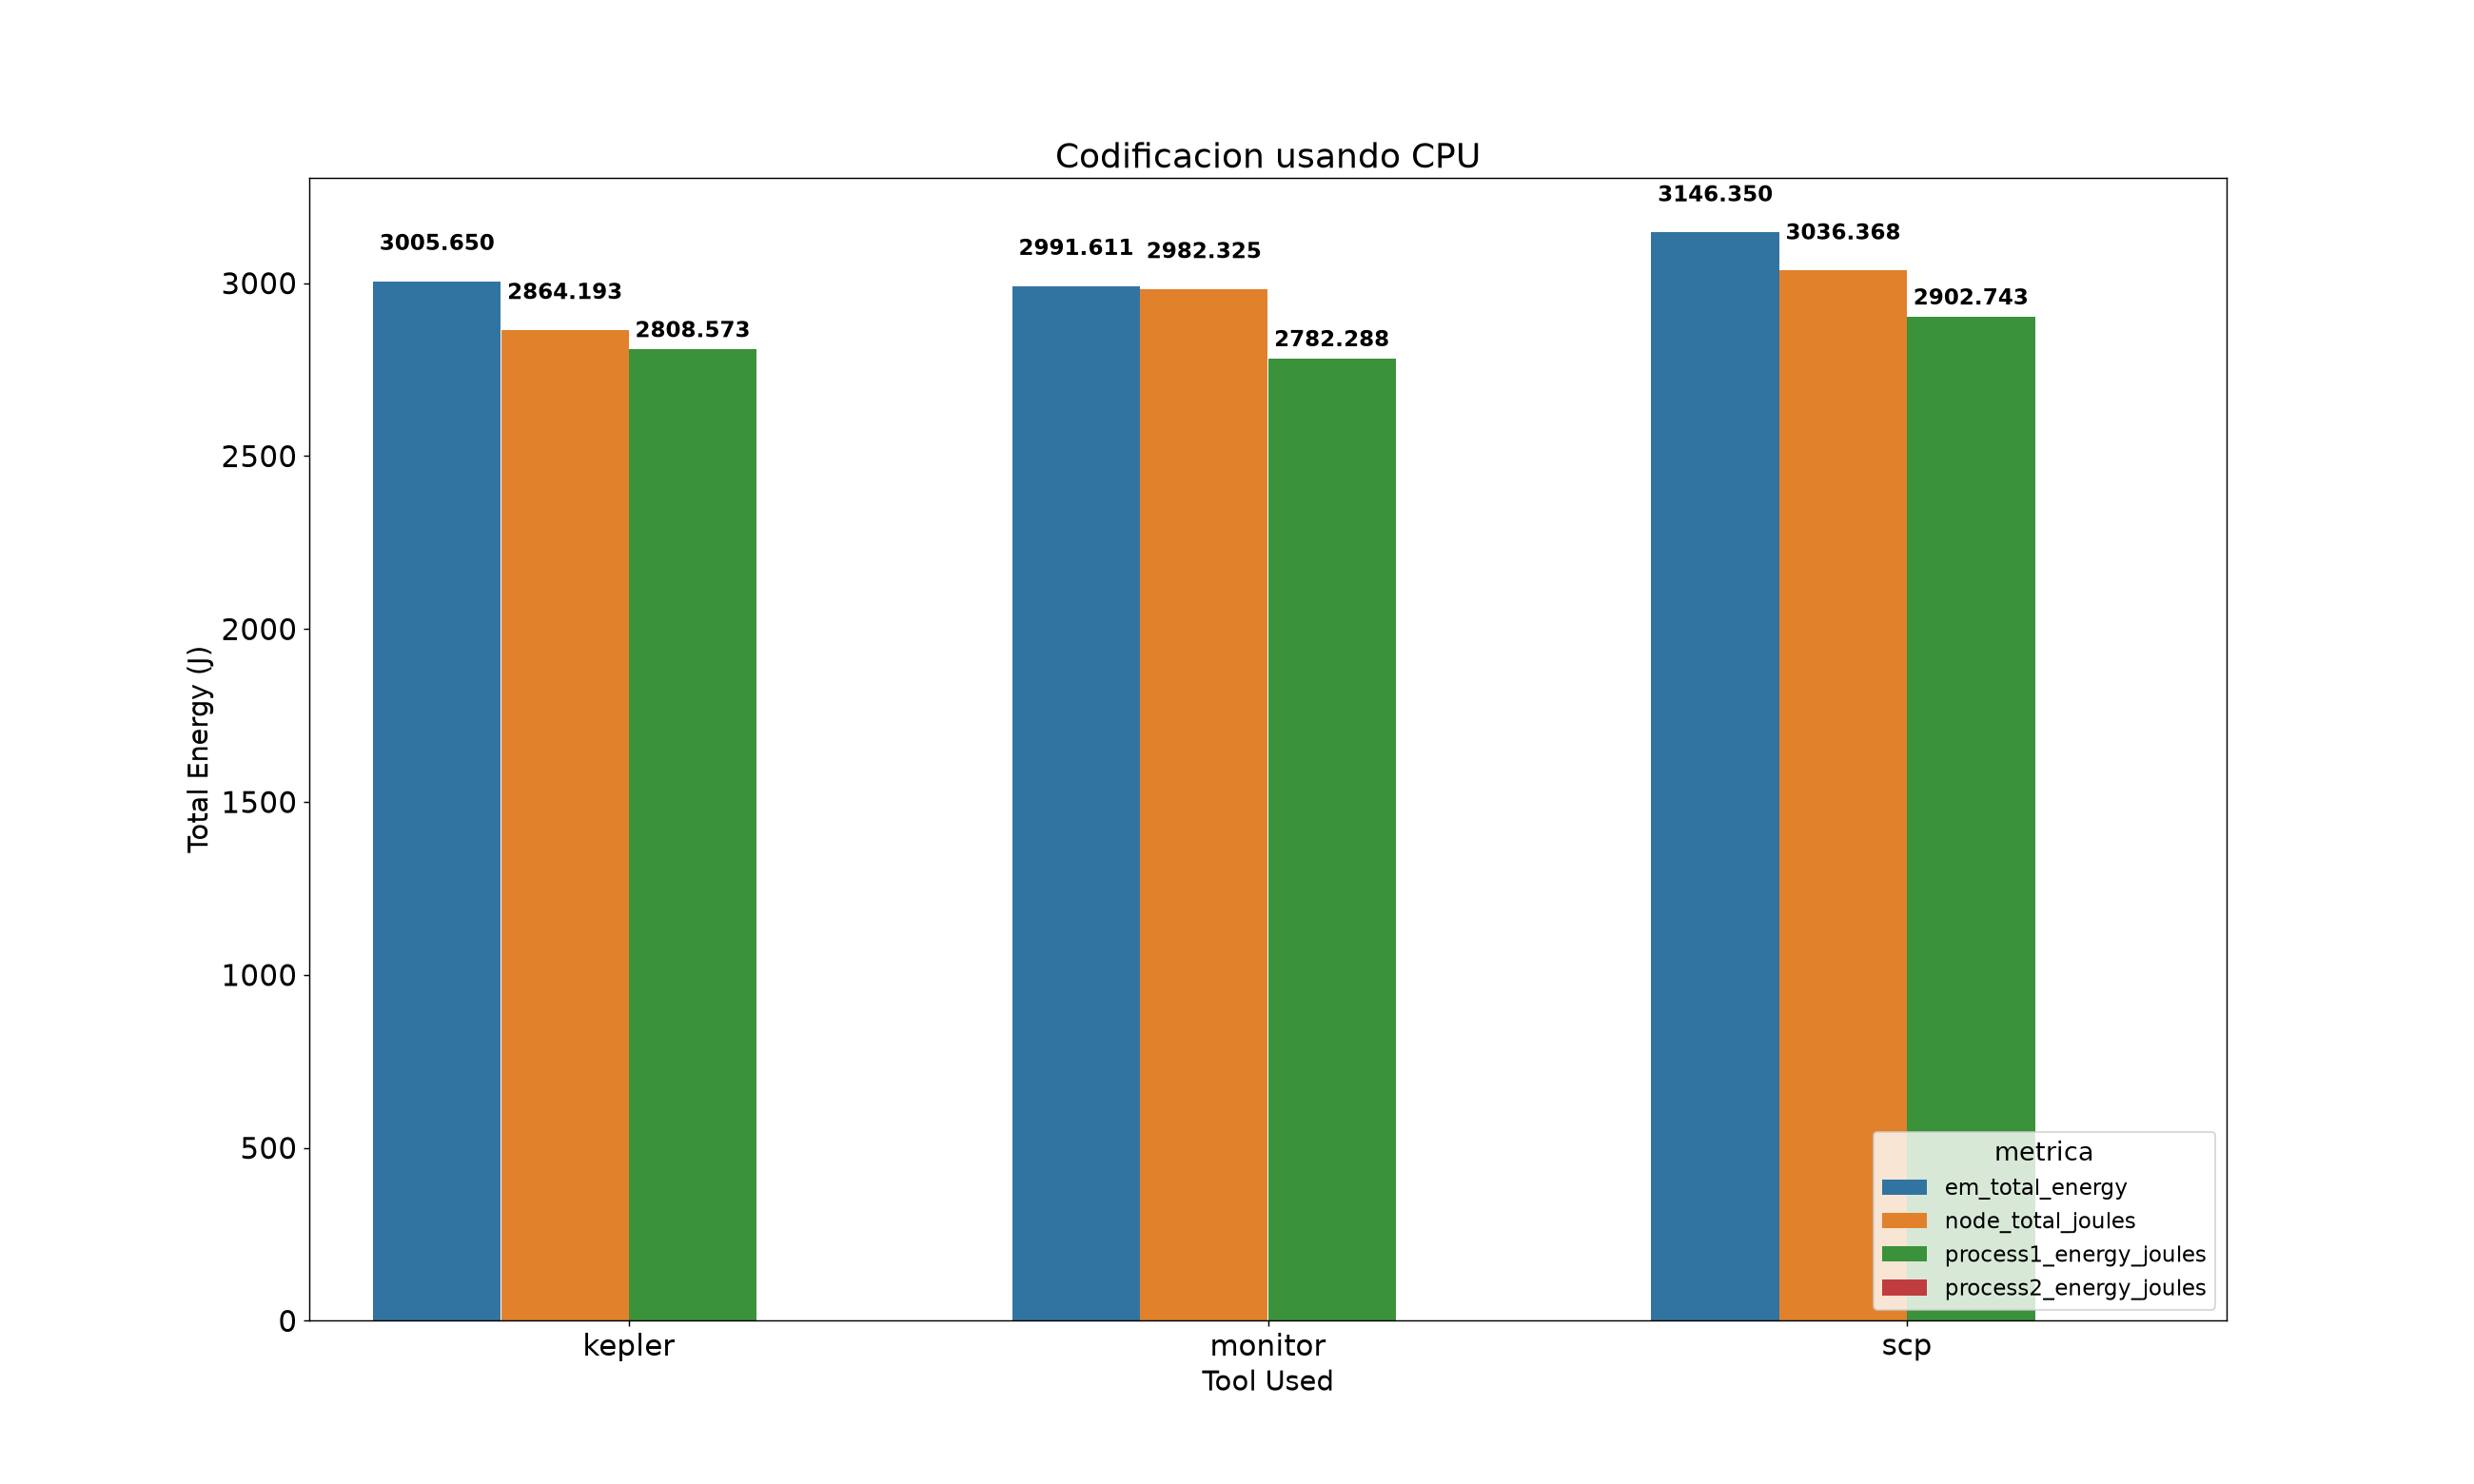
\includegraphics[width=\linewidth]{figs/exp1-1cont-nolimit.png}
    \caption{Histograma comparativo de las métricas de consumo energetico en julios de las tres herramientas sobre una tarea de transcodificacion llevada a cabo en un contenedore de docker (process1\_energy\_joules)}
    \label{fig:exp1-es2-resultados}
 \end{figure}

\subsubsection{Escenario 2: Transcodificación sobre un contenedor empleando CPU y GPU}
  En este escenario se le da acceso al contenedor tanto a la GPU como al numero total de cores de la CPU. Con esta comparativa se espera poder medir las capacidades basicas de cada una de las herramientas al tratar de determinar el consumo del nodo y de la GPU, asi como del proceso que se estan ejecutando sobre este en comparacion a las métricas de energia recolectadas por la herramienta externa Global Energy Meter.
  
  Cabe destacar que la energía total medida por \textit{Global Energy Meter} (\textbf{em\_total\_energy}) y por las herramientas de métricas respecto al nodo (\textbf{node\_total\_joules}) miden el consumo energético basándose en RAPL, lo cual implica que ninguna de estas medidas incluye el consumo de la tarjeta gráfica. Por tanto, para conocer el consumo total del sistema durante el proceso de codificación empleando tarjeta gráfica, se deben sumar las métricas de consumo del nodo y la métrica de consumo de la GPU (\textbf{gpu\_node\_jouls}) \(\textbf{gpu\_node\_jouls}+\textbf{em\_total\_energy} = \textbf{Total\_Energy\_System}\).
 
  En cuanto a la capacidad de tomar métricas de las herramientas, se observa que Scaphandre es la única herramienta que no ha sido capaz de tomar métricas de consumo energético de la GPU. En cambio, tanto Kepler como Container Energy Monitoring sí que han sido capaces de medir el consumo energético, siendo en ambos casos bastante similares. Esto nos sirve de indicativo de que el hotfix realizado sobre Kepler se comporta segun la referencia de consumo esperada, ademas de indicar que la capacidad de tomar métricas de consumo de la tarjeta gráfica de ambas herramientas parece ser adecuada.
 
  Si nos centramos en la capacidad para medir el consumo energético del nodo, Container Energy Monitoring es la que menor discrepancia presenta respecto a la energía que Global Energy Meter ha tomado del sistema, con una tasa de error del \textbf{$0,41\%$} calculada empleando la formula \ref{eq:percent-energy-node}. Seguida por Scaphandre quien presenta una tasa de error del 	\textbf{$3,06\%$}, y , en ultimo lugar, Kepler quien presenta un tasa de error del \textbf{$7,45\%$}.
 
  \begin{figure}[h!]
     \centering
     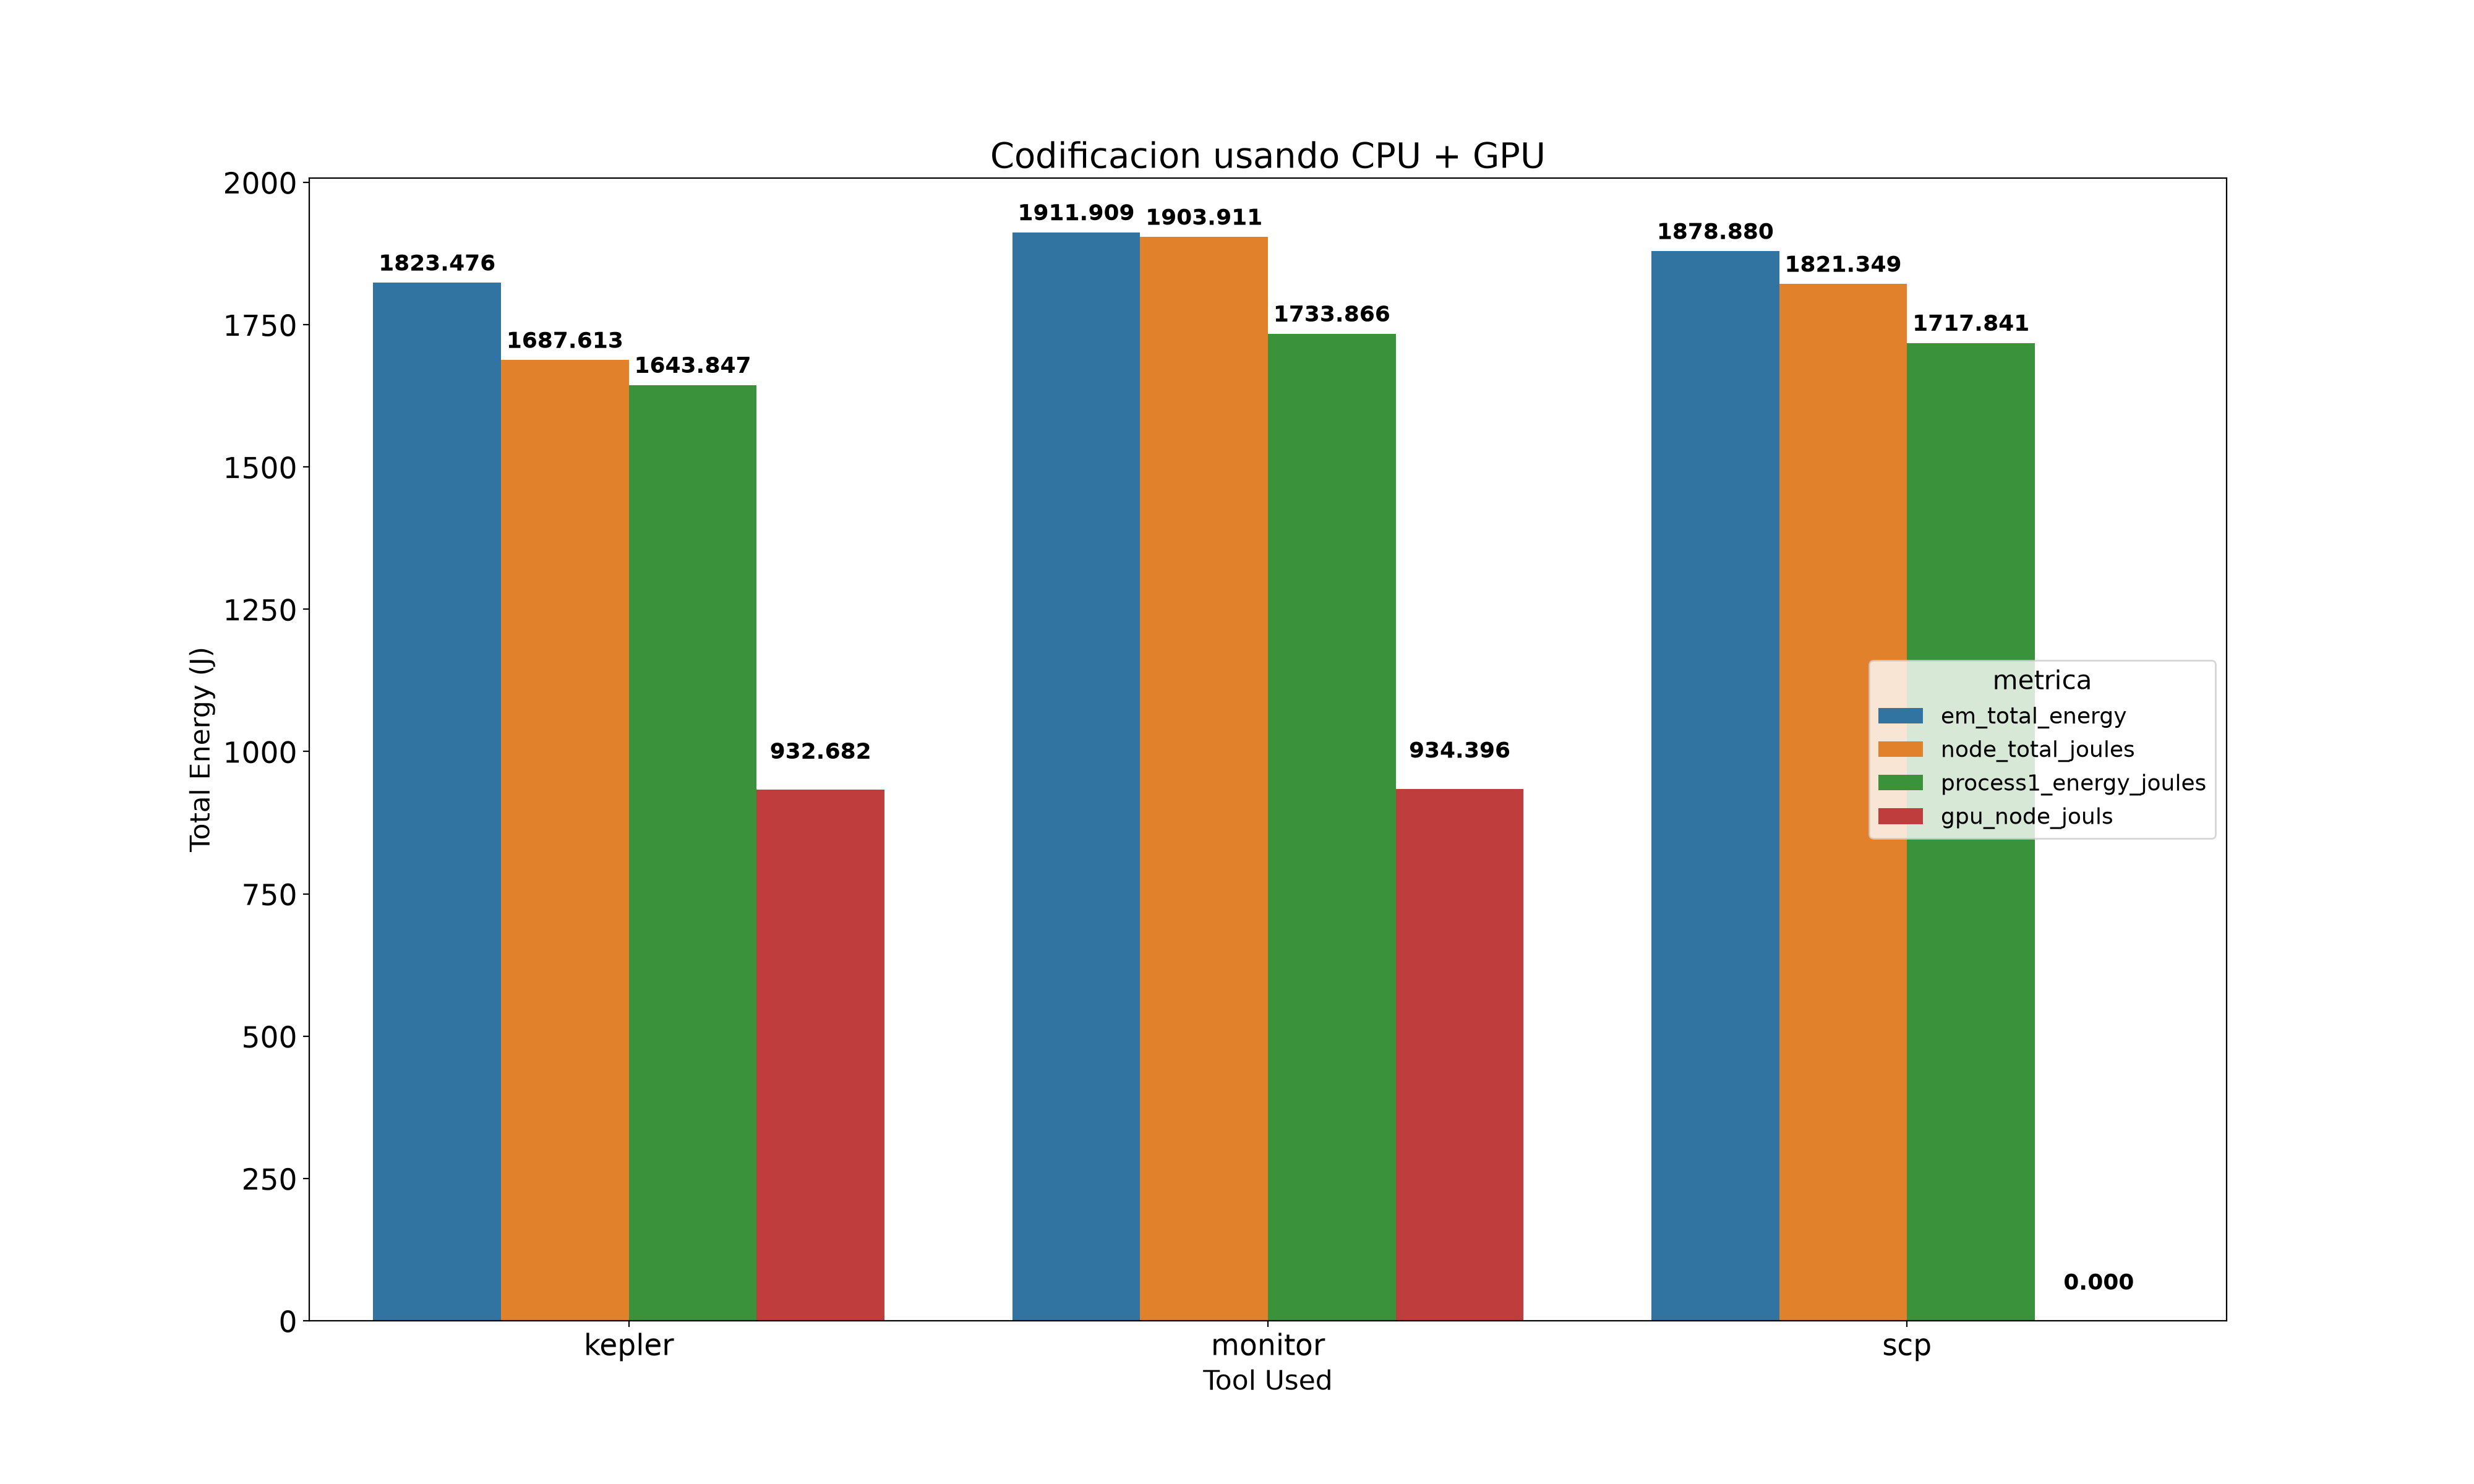
\includegraphics[width=\linewidth]{figs/exp1-1cont-nolimitcpuygpu.png}
     \caption{Histograma resultante de las métricas de consumo energetico en julios sobre una tarea de codificación empleando GPU y CPU}
     \label{fig:exp1-es1-resultados}
  \end{figure}


\subsubsection{Escenario 3: Transcodificacion empleando un contenedor limitado a tres cores}
 En este tercer escenario, se ha limitado el numero de cores a los que el contenedor tiene acceso con el fin de medir la granularidad de cada una de las herramientas en relacion a las métricas de consumo. Para limitar el numero de cores se han añadido las opciones:
 \begin{itemize} 
  \item \texttt{\lstinline[language=sh]{--cpus="3"}}: Numero de cores que el contenedor puede utilizar.
  \item \texttt{\lstinline[language=sh]{--cpuset-cpus=1-3}}: Rango de las cores de las que dispone, en este caso reservamos los cores \textit{0,4,5,6 y 7} para el sistema.
 \end{itemize}
 
 Analizando el consumo energetico general de las diferentes métricas, se observa un aumento del consumo energetico del \textbf{$31,99\%$} respecto al escenario que no presentaba limitacion en el numero de cores de la CPU. En cuanto a la metrica de consumo energetico del nodo, Container Energy Monitoring es el que menor discrepancia tiene respecto a la energia medida por Global Energy Meter con una tasa de error del \textbf{$0,2546\%$}. Seguido por Scaphandre, quien presenta un tasa de error del \textbf{$2,5921\%$} respecto a la energia medida por Global Energy Meter, y en ultimo lugar, Kepler el cual presenta un tasa de error del \textbf{$62,5930\%$}, una gran diferencia respecto tasa de error de las dos herramientas.
 
 Los resultados muestran que Container Energy Monitor es la herramienta que mejor atribuye la energía en el caso se que limite el número de cores asignados al contenedor. En este mismo escenario, Kepler y Scaphandre dan un valor muy bajo a la energía consumida por el contenedor. Para determinar las causas habría que analizar el código fuente, lo que queda fuera del ámbito de este trabajo.

 \begin{figure}[h!]
   \centering
   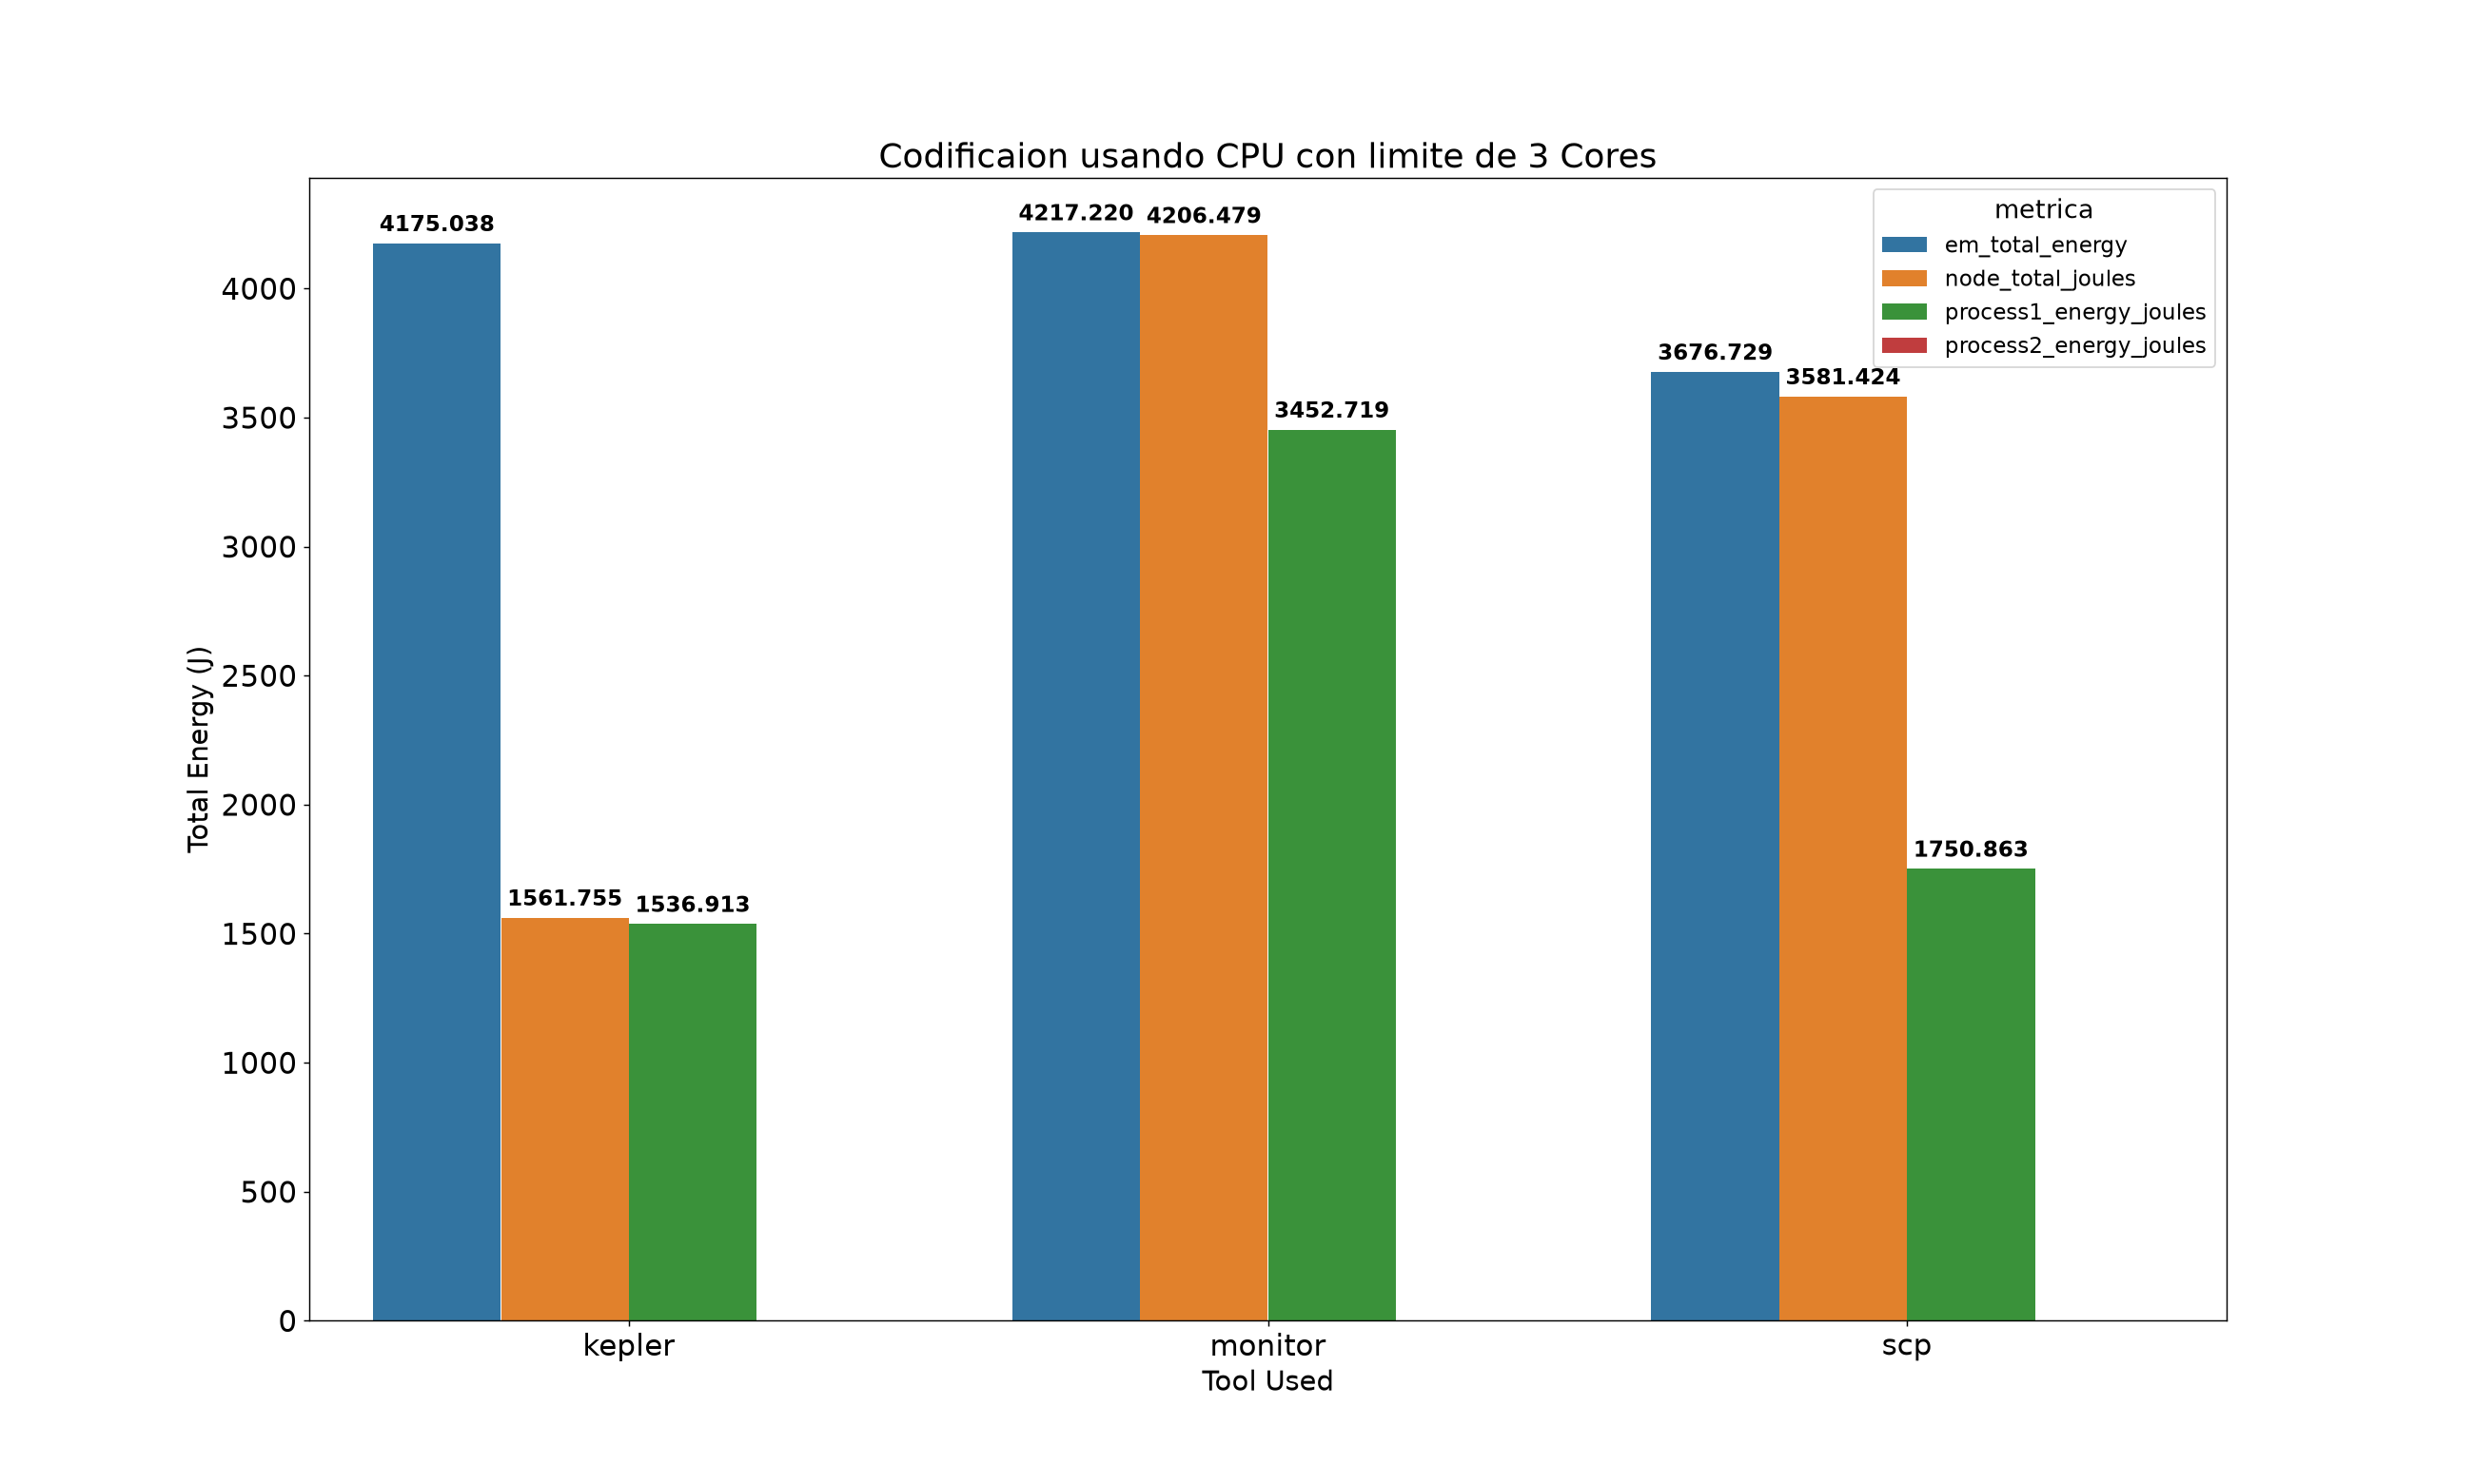
\includegraphics[width=\linewidth]{figs/exp1-1cont-limited3cpus.png}
   \caption{Histograma resultante delas métricas de consumo sobre una tarea de codificacion emplendo un contenedor limitado a 3 cores}
   \label{fig:exp1-es3-resultados}
 \end{figure}

\subsubsection{Escenario 4: Transcodificacion concurrente empleando dos contenedores limitados a tres cores cada uno}
 Finalmente, en el cuarto escenario experimental se limita el acceso a los recursos disponibles, distribuyendo la carga de trabajo entre dos contenedores. A cada contenedor se le asignan tres núcleos de CPU, reservando nuevamente los núcleos 0 y 7 para el sistema operativo. De este modo, el primer contenedor utiliza los núcleos 1--3, mientras que el segundo utiliza los núcleos \textit{4--6}. En este escenario, se van a usar el codificador que usa exclusivamente la CPU.
 
 En esta última fase se pretende evaluar la precisión y granularidad de las herramientas al monitorizar de forma simultánea el consumo energético asociado a dos contenedores que ejecutan procesos de transcodificación independientes. Los resultados obtenidos se muestran en la Figura \ref{fig:exp1-es4-resultados}.
 
 En relación a la estimacion de consumo energético respecto a la energia del nodo, \textbf{Container Energy Monitoring} presenta los resultados más próximos a la referencia obtenida mediante Global Energy Meter, con una tasa de error del \textbf{$0,5428\%$}. Seguido de Scaphandre, cuya medición presenta una diferencia de aproximadamente \textbf{200-300 julios}, lo que supone una tasa de error del \textbf{$2,9988\%$}, respecto a dicha referencia. En el caso de Kepler, se observa una discrepancia considerable en la estimación del consumo energético del nodo, con una tasa de error del \textbf{$25,1623\%$}. 
 
 Si se analiza específicamente el consumo energético atribuido a a los dos procesos de transcodificación, \textbf{Scaphandre} proporciona una estimación total de \textbf{$4653,025$ julios}. Por otro lado, el consumo energético medido por  Global Energy Meter asciende a \textbf{$6815,315$ julios}. Por tanto, se calcula \ref{eq:percent-energy-tool_node} que el consumo atribuido a los procesos representa aproximadamente el \textbf{$68,2730\%$} del consumo total estimado para el nodo. Es decir, las dos cargas principales de trabajo son los procesos de codificación y según esta herramienta un \textbf{30\%} de la energía (unos $2\,000$ julios) no se atribuye a estos procesos.
 
 Por su parte, Container Energy Monitoring proporciona una estimación del consumo energético asociado a los procesos cuya suma asciende a \textbf{$6212,860$ julios}, frente a un consumo energético medido por  Global Energy Meter de \textbf{$6733,879$ julios}. Esto supone una diferencia de \textbf{$521,019$ julios} y significa que \textbf{Container Energy Monitoring} atribuye aproximadamente el \textbf{$92,2627\%$} del consumo energético total del nodo a los procesos ejecutados en los dos contenedores. Este resultado es coherente con las condiciones del escenario descrito anteriormente, en el que la mayor parte de la carga de trabajo del sistema corresponde a los procesos de transcodificación ejecutados simultáneamente en ambos contenedores.

 En el el caso de la métricas tomadas por \textbf{Kepler}, se obtiene que ambos procesos han consumido un total de $4943,986$ julios mientras que Global Energy Meter indica que el nodo ha consumido $6694,905$ julios. Esto implica que kepler atribuye un \textbf{$73,8469\%$} de energia a los procesos de transcodificación. Esto implica que segun esta herramienta un \textbf{$26,19\%$} de la energia no se asigna a ningun proceso.


 \begin{figure}[h!]
     \centering
     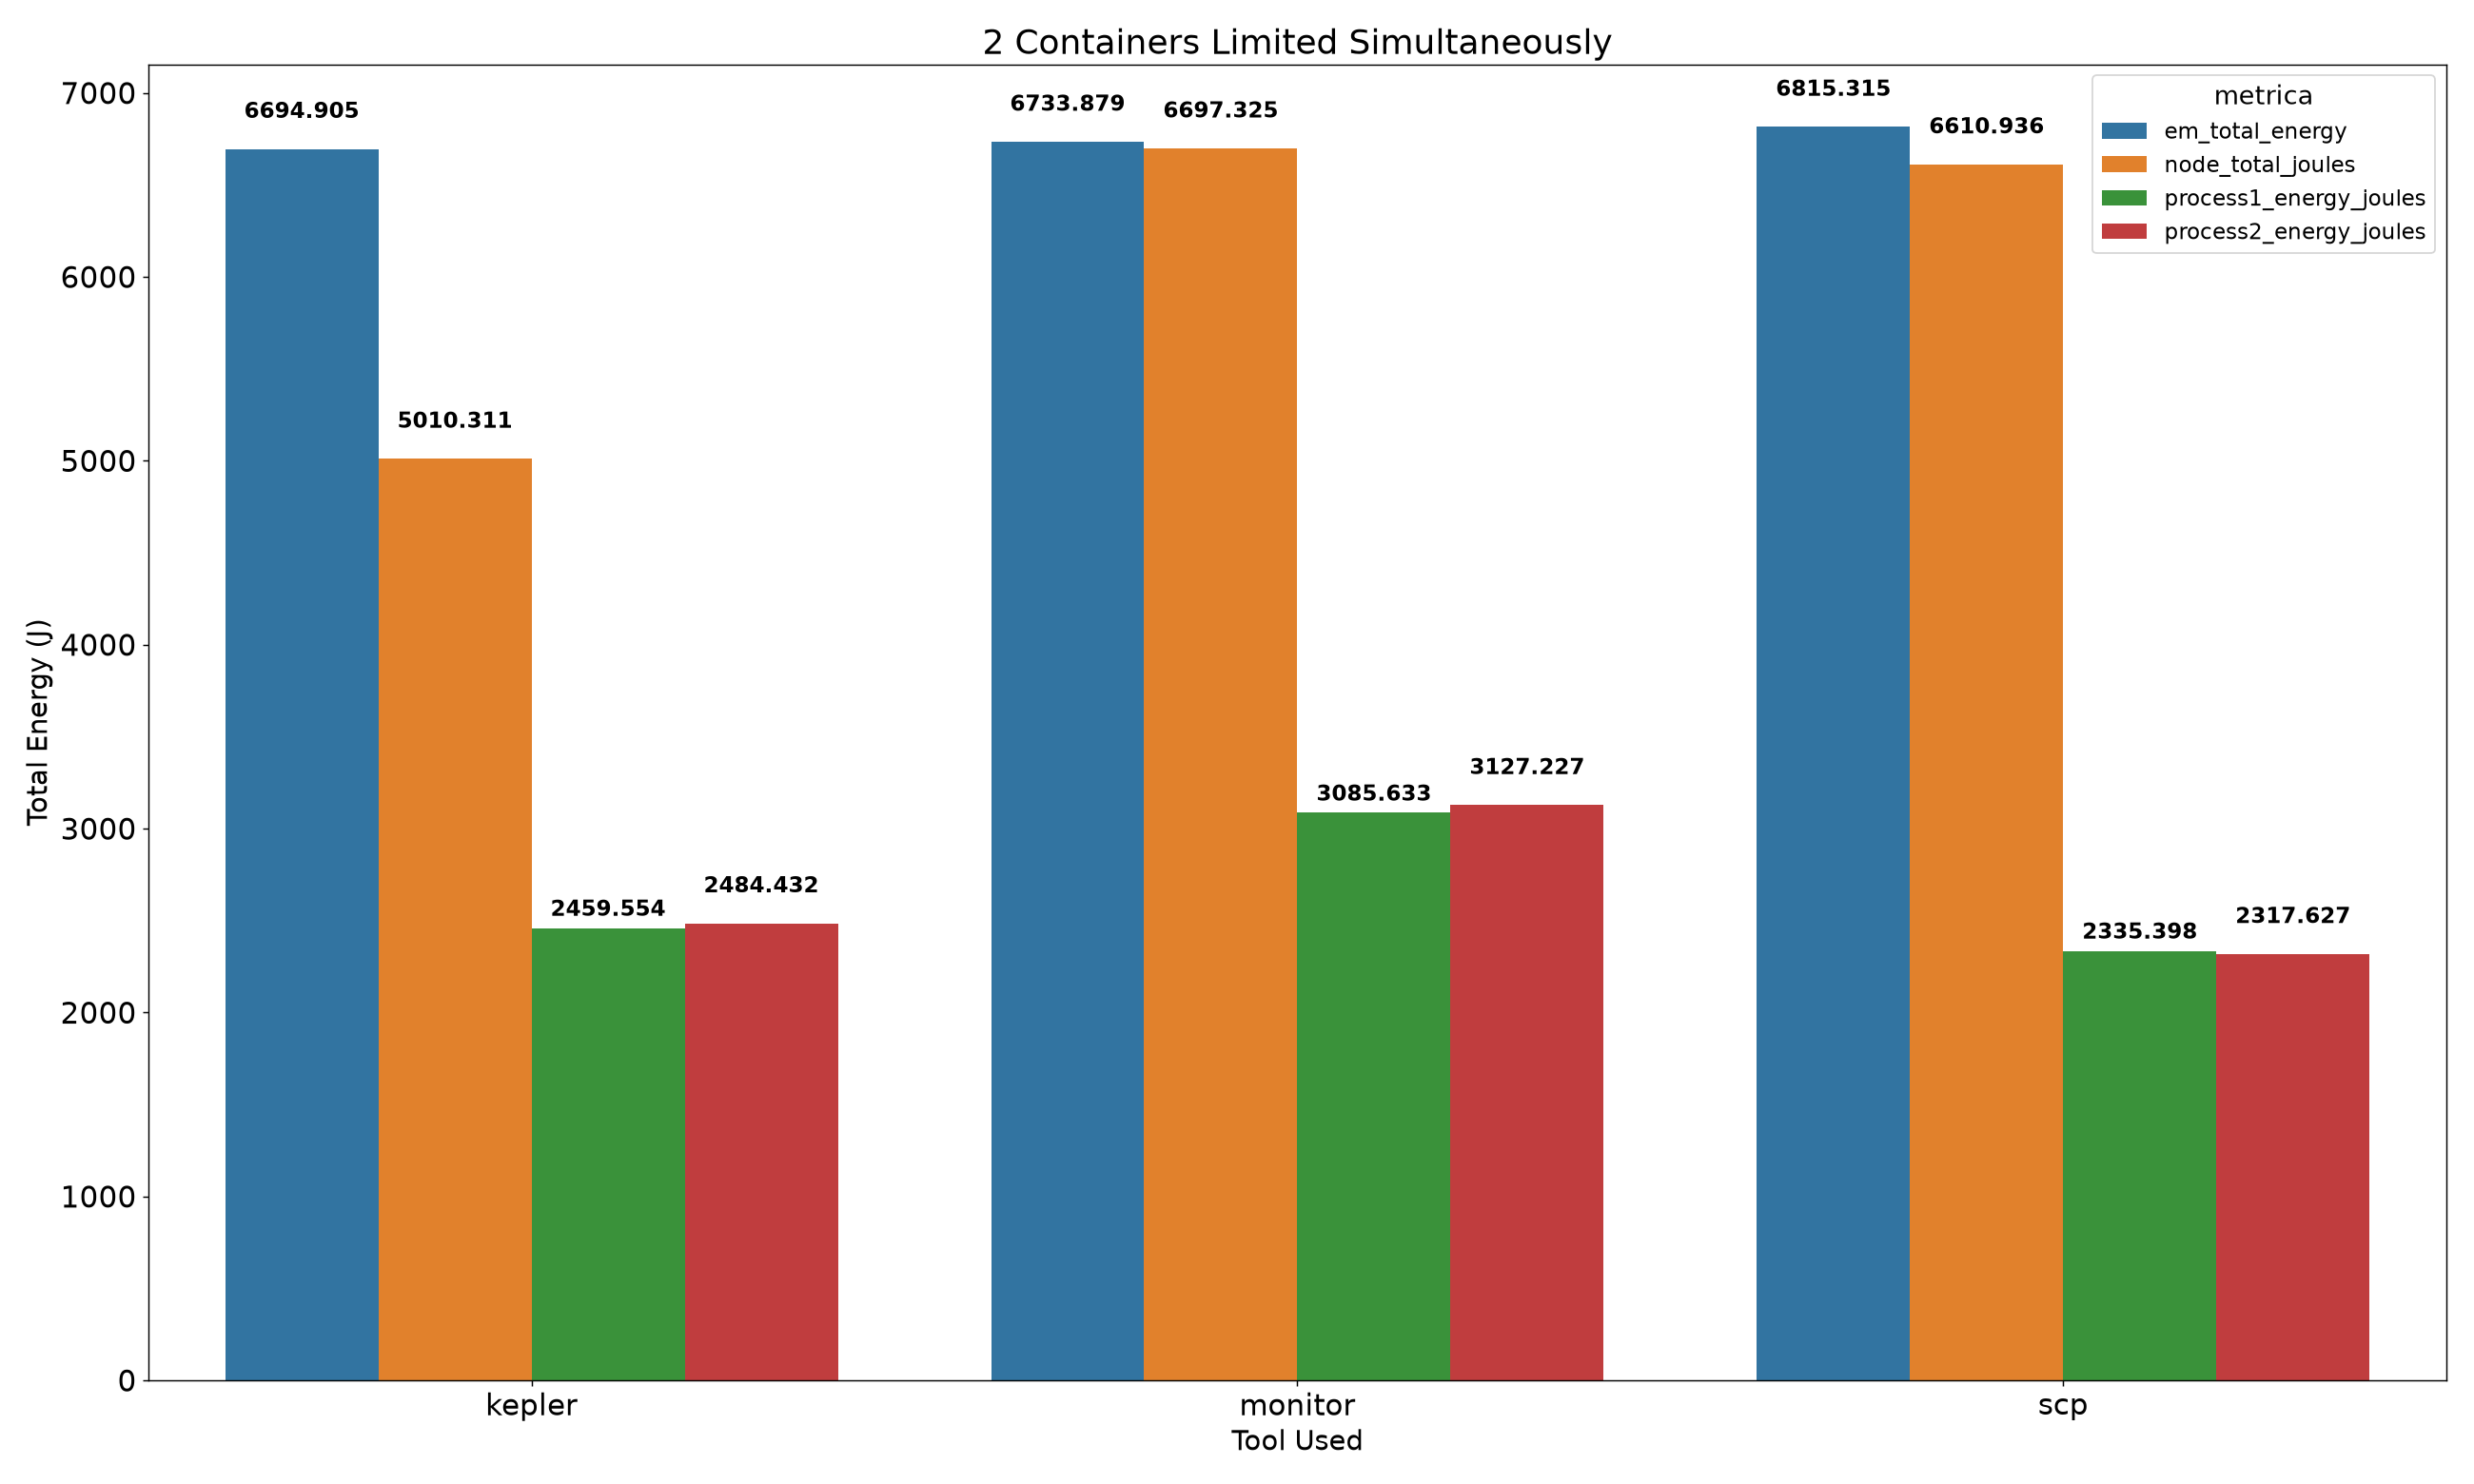
\includegraphics[width=\linewidth]{figs/exp1-2cont-limited3cpus.png}
     \caption{Histograma resultante de las métricas de consumo de dos contenedores limitados a 3 cores cada uno ejecutando tareas de codificacion simultaneamente}
     \label{fig:exp1-es4-resultados}
 \end{figure}

\subsection{Conclusiones fase 1 de la experimentacion }

Los experimentos llevados a cabo en esta primera fase han permitido comparar el comportamiento de \textit{Scaphandre}, \textit{Kepler} y \textit{Container Energy Monitoring} bajo distintas condiciones de ejecución, teniendo en cuenta tanto el consumo energético total del nodo como la posibilidad de atribuir dicho consumo a los procesos monitorizados. Los resultados obtenidos muestran diferencias importantes entre las herramientas, especialmente en situaciones donde se limitan diferentes recursos del sistema y se varía la carga de trabajo e incluso el número de procesos que se ejecutan al mismo tiempo.

En cuanto a la estimación del consumo energético del nodo, \textit{Container Energy Monitoring} es el que menor discrepancia respecto a la medida de referencia utilizada presenta, de forma general. En los escenarios estudiados, los errores obtenidos por esta herramienta se mantienen en valores bajos, llegando a un error del \textbf{0.25\%} en el escenario 3 y un error del \textbf{0.31\%} en el escenario 2. Scaphandre también da estimaciones cercanas a las de referencia en algunos casos, pero tiene mayor diferencia en el escenario 4. Por su parte, Kepler presenta un comportamiento más variable, alcanzando un error del \textbf{62.59\%} en el escenario 3.

Además de la estimación del consumo del nodo, la capacidad de desagregar el consumo entre las cargas de trabajo constituye un aspecto especialmente relevante para los objetivos de este trabajo. En este sentido, \textbf{Container Energy Monitoring} presenta una mayor capacidad de atribución del consumo energético a los procesos monitorizados. Esto resulta especialmente significativo en el escenario 4, donde consigue atribuir a los procesos el \textbf{92.77\%} del consumo total medido para el nodo, frente al \textbf{70.40\%} obtenido por Scaphandre y el \textbf{22.37\%} obtenido por Kepler. Por tanto, Contanier Energy Meter es la herramienta que mejor consigue estimar la energía en un escenario donde hay concurrencia de procesos y los contenedores tienen recursos limitados.

\begin{table}[htbp]
     \centering
     \begin{tabularx}{\textwidth}{|>{\raggedright\arraybackslash}X|r|r|r|}
     \hline
     \rowcolor[HTML]{C0C0C0} 
     Herramienta & \multicolumn{1}{c|}{GEM (j)} & \multicolumn{1}{c|}{Energia del Procesos (j)} & \multicolumn{1}{c|}{Energía Sin Atribuir (\%)} \\ \hline
     Global Energy Monitor & 6733,879 & 6212,860 & 7,73 \\ \hline
     Scaphandre & 6815,315 & 4653,025 & 31,73 \\ \hline
     Kepler & 6694,905 & 4940,98 & 26,19 \\ \hline
     \end{tabularx}
     \caption{Tabla comparativa de las métricas de consumo de los procesos de codificación obtenidos por cada herramienta, junto con el porcentaje de energía sin atribuir frente a la energía medida en cada caso por Global Energy Meter.}
     \label{tab:exp1-conclusiones-esc4}
\end{table}

Por otra parte, los resultados alcanzados posibilitan la identificación de ciertas limitaciones de las herramientas evaluadas. Scaphandre tiene ciertas limitaciones a la hora de obtener información energética relacionada con algunos recursos de hardware, como la GPU. También tiene limitación a la hora de tomar métricas sobre múltiples procesos sobre múltiples contenedores en simultáneo, ya que, como se puede observar en la tabla comparativa \ref{tab:exp1-conclusiones-error}, el error respecto a la energía medida por EM escala conforme al número de procesos aumenta.  

En el caso de Kepler, si bien no tiene problemas para medir el consumo sobre la GPU, presenta discrepancias importantes a la hora de estimar el consumo energético del nodo, con un gran nivel de error, lo que restringe su elección como herramienta de toma de métricas de uno o varios procesos del sistema. Este factor dificulta la posibilidad de saber si las métricas recolectadas del conjunto de procesos están sobreestimadas o, por el contrario, muy por debajo del consumo real.

Estas diferencias muestran que es importante seleccionar la herramienta no solo por su capacidad de obtener una medida energética, sino también por la granularidad y nivel de atribución que ofrece.

Por lo tanto, y teniendo en cuenta la discrepancia respecto a la referencia, la capacidad de atribución del consumo a los procesos y el comportamiento observado en los distintos escenarios, se selecciona Container Energy Monitoring como herramienta para las siguientes fases del estudio. Esta selección facilitará una mayor precisión en la medición del consumo energético de las cargas de trabajo implementadas, elemento clave para posteriormente examinar el impacto energético de los diferentes escenarios de transcodificación estudiados en este trabajo.

\begin{table}[ht!]
     \centering
     \begin{tabularx}{\textwidth}{|>{\raggedright\arraybackslash}X|r|r|r|r|}
     \hline
     \rowcolor[HTML]{C0C0C0} 
     Herramientas & ES1 & ES2 & ES3 & ES4 \\ \hline
     \cellcolor[HTML]{EFEFEF}KEPLER & $4,685\%$ & $7,45\%$ & $62,593\%$ & $25,16\%$ \\ \hline
     \cellcolor[HTML]{EFEFEF}SCP & $3,4955\%$ & $3,06\%$ & $2,5921\%$ & $2,9988\%$ \\ \hline
     \cellcolor[HTML]{EFEFEF}Container Energy Monitor & $0,3113\%$ & $0,41\%$ & $0,2546\%$ & $0,5428\%$ \\ \hline
     \end{tabularx}
     \caption{Tasa de error de estimación de consumo energético en el nodo en comparación con la energía medida por Global Energy Meter en cada uno de los escenarios}
     \label{tab:exp1-conclusiones-error}
\end{table}

\label{exp1-desarrollo}
 \section{Experimento 2: Consumo energético en relación con el SITI}       
 El objetivo principal de este experimento es tratar de encontrar una relación entre las características de video, Spatial Information (SI) y Temporal Information (TI), y el consumo energético necesario para llevar a cabo un proceso de transcodificación de video. 

 Para poder llevar a cabo el experimento 2 con éxito, previamente se debe realizar una clasificación de los videos del dataset en base a los valores del SI y el TI. Es por ello que esta sección se ha dividido en dos subsecciones que expondrán cómo se han llevado a cabo cada uno de los experimentos y el postprocesamiento de los datos.

 Finalmente, el análisis de las gráficas y conclusiones del experimento 2, se llevará a cabo en la sección \textit{Resultados del Experimento 2.2: Consumo energético en relación al SITI} \ref{subsec:exp2.2-siti}. 

 En cuanto a los experimentos, se han empleado un total de cuatro codificadores; dos de ellos basados en codificación mediante CPU (libx264 y libx265); y otros dos que combinan la CPU junto con la GPU (h264\_nvenc y hevc\_nvec). 

 También se ha variado el bitrate en cada transcodificación de cada video, y dependiendo de si se trataba de un codec del estándar H.264 o del estándar H.265, se ha empleado una lista de bitrates concreta. La selección de dichos rangos de bitrate, se ha hecho en base a las recomendaciones \cite{bitrate-encoder-selection}, y posteriormente se ha aumentado el rango del bitrate máximo y mínimo con el fin de remarcar diferencias fácilmente apreciables en el resultado final de codificación y, simultáneamente, medir el esfuerzo requerido por el codec conforme el bitrate aumenta. Los rangos de bitrate (en Mb por segundo) empleados son:

\begin{itemize} 

 \item \texttt{libx264 y H264\_NVENC}: 10,20,25,30,35,40,50

 \item \texttt{libx265 y H265\_NVENC}: 10,15,20,25,30,35,40   

 \end{itemize}

Por tanto, se ha transcodificado cada video empleando los codificadores y los bitrates correspondientes de la lista, midiendo cada proceso con la herramienta seleccionada en el Experimento 1 (Container Energy Monitoring). 

En ambas fases se ejecutará únicamente un contenedor por prueba, sin concurrencia de procesos o contenedores, basado en la imagen \textbf{linuxserver/ffmpeg:8.0.1}. El resto de parámetros de la declaración del contenedor son idénticos en cada subfase, a diferencia del nombre y del número de CPU disponibles, ya que, al contrario que en la fase 1, en la fase 2 sí que se limita el número de contenedores de la misma forma que en la sección \ref{exp1-desarrollo}.

\begin{lstlisting}[language=sh,caption={Declaracion de container básica para las pruebas de la subfase 1 y subfase 2}]

  #Sin limitaciones

  docker run -d --name ffmpeg-encoder --network global_monitoring_default -v "$(pwd)/VIDEOS":/config --runtime=nvidia --entrypoint sleep linuxserver/ffmpeg:8.0.1 18000

  #Limitao a X cores de Y a Z

  docker run -d --name ffmpeg-encoder --network global_monitoring_default --cpus="X" --cpuset-cpus="Y-Z" -v "$(pwd)/VIDEOS":/config --runtime=nvidia --entrypoint sleep linuxserver/ffmpeg:8.0.1 18000

\end{lstlisting}

En cuanto a los videos seleccionados para llevar a cabo los distintos experimentos, nuevamente, se ha empleado la base de datos de vídeos existente en el grupo de investigación. Se han utilizado videos compuestos por los chunks de los videos de la tabla \ref{tab:lista-videos-test}. En concreto, para los experimentos de esta sección, los vídeos estaban codificados utilizando el encoder libx264 con una resolución 4K (3840 x 2160) SDR, un CRF 0 y 30 fps. Destacar que tienen un perfil de color yuv420p (4:4:4) con una profundidad de 8 bits  \footnote{Profundidad de color obtenida con la orden de ffmpeg: \lstinline[language=sh, label={ffmpeg-achive-colordeep}]{ffprobe -v error -select_streams v:0 -count_frames -show_entries stream=nb_read_frames -of csv=p=0 VIDEO.mp4}} y 60 fotogramas por chunk \footnote{Número de frames del segmento de video obtenidos con la orden de ffmpeg: \lstinline[language=sh]{ffprobe -v error -select_streams v:0 -count_frames -show_entries stream=nb_read_frames -of csv=p=0 VIDEO.mp4}}.

\subsection{Experimento 2.1: Clasificación de chunks en base a los valores SI y TI}

Con el objetivo de establecer una correlación entre el consumo energético asociado al proceso de codificación de vídeo y las métricas \textit{Spatial Information} (SI) y \textit{Temporal Information} (TI), se definieron cuatro categorías en función de los valores de SI y TI. Posteriormente, se seleccionó una serie de \textit{chunks} en función de sus valores potenciales de SI y TI, tomando como referencia tanto la visualización de los vídeos como los datos obtenidos del trabajo de Tesis de Francisco Miguel Micó Enguídanos.

Cabe destacar que, aunque el conjunto de datos contiene los valores de SI y TI calculados para todos los chunks del conjunto de vídeos utilizado en los experimentos, dichos valores no pudieron emplearse directamente, ya que fueron obtenidos utilizando una versión anterior\footnote{https://www.itu.int/rec/T-REC-P.910-202310-I/en} del estándar SITI. Para este trabajo, los valores de SI y TI se calcularon siguiendo el nuevo estándar \textbf{P.910 (07/26)}\footnote{https://www.itu.int/rec/T-REC-P.910-202607-P/en}.

Por este motivo, se desarrolló el script \textbf{exp2.1-siticalculator} (Apédice \ref{code:script-siti-calculation} \ref{code:script-siti-calculation-obj} ) en Python, que hace uso de la librería \textit{SITI Tool} \cite{siti-tool-pypip} para calcular los valores de SI y TI de cada \textit{chunk}. Posteriormente, el script procesó los resultados obtenidos y los almacenó en un archivo CSV con la estructura mostrada en (Apéndice \ref{fig:exp2.1-sititool-header-csv}).

\dosubfigs
     {figs/exp2.1-siti-pacomico.png}{Ubicación de chunks de video en base a los datos de F. Micó}{fig:exp2.1-chunks-data-pacomico}
     {figs/exp2.1-ChucnkSITI-01.png}{Posición de los chunks en base a las características SI y TI}{fig:exp2.1-chunks-combined}

Una vez determinada la posición de cada \textit{chunk} en función de sus valores de SI y TI, se definieron las cuatro zonas utilizadas para su clasificación, estableciendo para cada una de ellas los correspondientes rangos de SI y TI. El resultado de esta clasificación se recoge en la tabla \ref{tab:siti-zones-definition}.

Cabe destacar que la definición de los límites de cada zona presentó cierta dificultad, debido a que una gran parte de los chunks se concentra en la zona media-central del espacio SI-TI. Por este motivo, los rangos establecidos para las diferentes zonas presentan valores relativamente próximos entre sí. Asimismo, se encontraron dificultades para obtener chunks con valores elevados de TI, ya que no se identificó ningún \textit{chunk} con un valor superior a 35. De forma similar, los valores de SI obtenidos no superaron el valor de 45.

\begin{table}[h]

     \centering

     \begin{tabular}{|c|ccc}

     \cline{1-1}

     \rowcolor[HTML]{9B9B9B} 

     \textbf{Categoria} & \textbf{Etiqueta de Referencia} & \textbf{SI} & \textbf{TI}                         \\ \hline

     Bajo SI y Bajo TI  & \multicolumn{1}{c|}{LSI\_LTI}   & \multicolumn{1}{c|}{\textgreater 5}  & \multicolumn{1}{c|}{\textgreater 5} \\ \hline

     Alto SI y Bajo TI  & \multicolumn{1}{c|}{HSI\_LTI}   & \multicolumn{1}{c|}{\textless 25}    & \multicolumn{1}{c|}{\textgreater 5} \\ \hline

     Bajo SI y Alto TI  & \multicolumn{1}{c|}{LSI\_HTI}   & \multicolumn{1}{c|}{\textgreater 10} & \multicolumn{1}{c|}{\textless 16}   \\ \hline

     Alto SI y Alto TI  & \multicolumn{1}{c|}{HSI\_HTI}   & \multicolumn{1}{c|}{\textless 15}    & \multicolumn{1}{c|}{\textless 8}    \\ \hline

     \end{tabular}
      \caption{Zonas de video para la clasificacion de chunks en base al SITI}
      \label{tab:siti-zones-definition}

\end{table}

\subsection{Experimento 2.2: Consumo energético en relación al SITI}\label{section:exp2.2-sitixconsumo}

En este primer subapartado se ha definido el conjunto de vídeos que se utilizará para analizar la relación entre el consumo energético asociado al proceso de codificación y los valores de las métricas \textbf{SI} y \textbf{TI}. Para ello, se requirieron vídeos de \textbf{10 segundos de duración} que no presentaran cambios de escena significativos ni cortes bruscos que pudieran alterar los valores medios de las métricas \textbf{SI} y \textbf{TI}. 

Para generar los vídeos utilizados en los experimentos, se siguieron dos estrategias diferentes. La primera estrategia consistió en seleccionar un único \textit{chunk} y reproducirlo de forma continua hasta alcanzar una duración de 10 segundos, utilizando ffmpeg de la siguiente forma \lstinline[language=sh,label={code:ffmpeg-loopvideo},caption={}]{ffmpeg -y -stream_loop 5 -i CHUNCKXXX.mp4 -t 10 -b:v 30000k -r 30 -c:v copy -an VIDEO_10S_CHUNCKXXX.mp4}. De esta forma, se evitó introducir cambios bruscos de escena y se mantuvieron las características espaciales y temporales del \textit{chunk} original. Cada vídeo generado se identificó mediante el nombre del vídeo de procedencia y el número del \textit{chunk} seleccionado.

La segunda estrategia consistió en generar un vídeo a partir de la concatenación de la mayor cantidad posible de \textit{chunks} pertenecientes a una misma zona, utilizando además los \textit{chunks} consecutivos correspondientes al vídeo original. Esta estrategia permitió reducir la variabilidad que pudiera derivarse de las características internas de optimización de cada códec durante el proceso de codificación. Los vídeos generados mediante esta estrategia se identificaron utilizando el nombre del vídeo original y el identificador del primer \textit{chunk} empleado, correspondiente al \textit{chunk} \textit{0000}.

En total, se seleccionaron \textit{cinco vídeos por zona}, a excepción de las zonas \textbf{HTI\_LSI}, habiendo añadido un vídeo más, y \textbf{HTI\_HSI}, habiendo añadido dos vídeos de más. Adicionalmente, se ha generado un video por zona empleando varios chunks, lo que ha resultado en una muestra final de \textit{28 vídeos}. Los resultados se muestran en la tabla \ref{tab:exp2.2-videos}.

\begin{table}[h!]

 \centering

 \small   % Reducimos un poco el tamaño de letra

 \begin{tabularx}{\textwidth}{|>{\centering\arraybackslash}X|>{\centering\arraybackslash}X|>{\centering\arraybackslash}X|>{\centering\arraybackslash}X|}

 \hline

 \rowcolor[HTML]{C0C0C0}

 \textbf{LSI\_LTI} & \textbf{HSI\_LTI} & \textbf{LSI\_HTI} & \textbf{HSI\_HTI} \\

 \hline

 LifeUntouched\_0053                 & Sintel\_0021                         & Eldorado\_0014                & Skateboarding\_0027                 \\ \hline

 LifeUntouched\_0055                 & Sintel\_0026                         & Eldorado\_0016                & Skateboarding\_0021                 \\ \hline

 LifeUntouched\_0048                 & Sintel\_0027                         & Eldorado\_0012                & Skateboarding\_0020                 \\ \hline

 LifeUntouched\_0075                 & IndoorSoccer\_0046                   & Eldorado\_0015                & Eldorado\_0011                      \\ \hline

 LifeUntouched\_0056                 & Sintel\_0022                         & IndoorSoccer\_0004            & Eldorado\_0010                      \\ \hline

 LifeUntouched\_0000 {[} 51 - 55 {]} & TearsOfSteel\_0235                   & Eldorado\_0000 {[} 12 - 16{]} & Sintel\_0091                        \\ \hline

 \textbf{-}                          & TearsOfSteel\_0234                   & \textbf{-}                    & Skateboarding\_0000 {[} 20 - 25 {]} \\ \hline

 \textbf{-}                          & TearsOfSteel\_0000 {[} 231 - 235 {]} & \textbf{-}                    & \textbf{-}                          \\ \hline

 \end{tabularx}

 \caption{Videos creados para la experimentación de consumo energético en relación con las características SITI}

 \label{tab:exp2.2-videos}

\end{table}

% SELECCION DE EXPERIMENTOS

La fase de experimentación se ha llevado a cabo empleando el script \textbf{exp2.2-sisti-energy.sh} (Apéndice \ref{code:exp2.2-sitienergy}), desarrollado en bash. Este lleva a cabo la transcodificación de cada uno de los vídeos seleccionados empleando con cada uno de los codificadores especificados en \ref{tab:exp2-codecs-selection}, junto con los correspondientes bitrates definidos para cada estándar de codificadores. Para los experimentos realizados en esta fase se utilizó un único contenedor, sin establecer restricciones sobre el número de CPU y/o núcleos disponibles.

El resultado de la toma de métricas de cada uno de los procesos de transcodificación es almacenado en la estructura de directorios mostrados en la Figura \ref{fig:exp2.2-datapath}, siendo el primero de todos el nombre del experimento. Esta estructura se diseñó con el objetivo de facilitar la automatización del procesamiento posterior de los datos mediante un script de Python.

\begin{figure}[H]

    \centering

    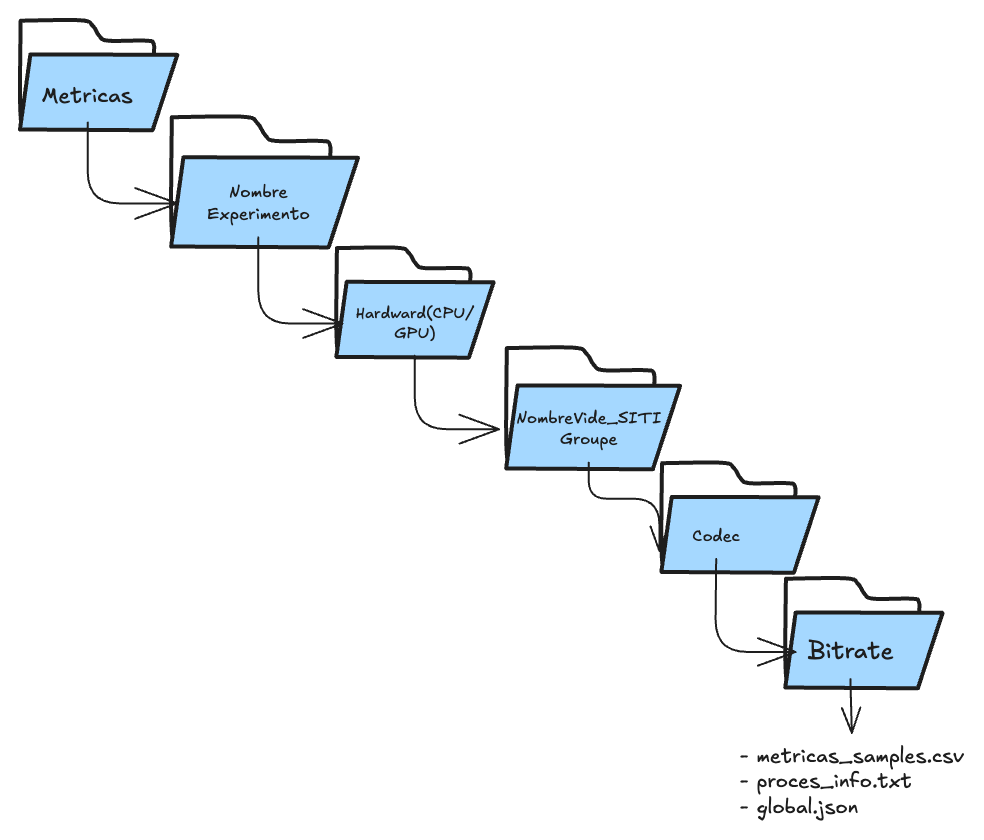
\includegraphics[width=0.3\linewidth]{figs/exp2.1-DataPathSITI.png}

    \caption{Árbol de directorios en el que se almacenan los datos de consumo energéticos de cada iteración}

    \label{fig:exp2.2-datapath}

\end{figure}

%POST-PROCESAMIENTO DATOS

El postprocesamiento de las métricas recopiladas se realizó mediante el script de Python \textbf{ploter-exp2.2.py} (Apéndice\ref{code:exp2.2-ploter} y \ref{code:exp2.2-ploter-obj}). Este script permite procesar y estructurar los datos obtenidos, almacenándolos en un archivo CSV con la estructura mostrada en \ref{fig:exp2.2-csvheader-dataprocess}. Asimismo, permite generar diferentes representaciones gráficas a partir de los datos procesados.

El script está diseñado para ejecutarse desde la interfaz de línea de comandos (\textit{CLI}), mediante diferentes \textit{flags} que permiten especificar tanto el tipo de procesamiento que se desea realizar como la ubicación de los datos de entrada \footnote{Ejecución básica del script \textbf{ploter-exp2.2.py} \lstinline[language=sh]{python3 ploter-exp2.2.py NOMBRE-EXPERIMENTO [FLAGS]}}. Las opciones que acepta el script (tanto opcionales como obligatorias) pueden apreciarse a continuación: 

\begin{itemize}
     \item \textbf{process}: Permite procesar las métricas de consumo obtenidas durante el experimento \textit{exp2.2}. Por defecto, el script accede al directorio \textit{AllMetrics}, aunque es posible especificar una ruta alternativa.

     \item \textbf{plot3d}: Permite representar la posición de cada vídeo en un gráfico tridimensional, en el que el eje X representa el valor de TI, el eje Y el valor de SI y el eje Z el consumo energético del contenedor. Se genera una gráfica para cada combinación de codificador y \textit{bitrate}.

     \item \textbf{plot-consumo-ti}: Permite generar una gráfica bidimensional de tipo \textit{stream} para cada combinación de codificador y \textit{bitrate}. En este caso, el eje X representa el valor de TI y el eje Y el consumo energético, expresado en julios, del proceso de transcodificación.

     \item \textbf{plot-consumo-si}: Permite generar una gráfica bidimensional de tipo \textit{stream} para cada combinación de codificador y \textit{bitrate}. En este caso, el eje X representa el valor de SI y el eje Y el consumo energético, expresado en julios, del proceso de transcodificación.
     
     \item \textbf{plot-consumoxtiempo-grupal}: Permite generar una gráfica de dispersión de puntos, los cuales se agrupan por codec y bitrate utilizado. En este caso lleva a cabo una comparativa entre consumo energético y tiempo de codificación, permitiendo discernir cómo afectan las características de los videos.

     \item \textbf{--data-final-dir=PATH\_ARCHIVO}: Permite definir una ruta alternativa para almacenar el archivo CSV resultante del procesamiento de los datos. Por defecto, se utiliza la ruta \textit{./data/ex2.2\_process\_data.csv}.

     \item \textbf{--container=consumo\_container0\_j}: Permite seleccionar el contenedor cuyos datos de consumo se utilizarán para generar las gráficas, en caso de que se hayan ejecutado varios contenedores. Por defecto, se utilizan los datos correspondientes a la columna \textit{consumo\_container0\_j}.

\end{itemize}

\subsection{Resultados del Experimento 2: Consumo energético en relación al SITI}\label{subsec:exp2.2-siti}
 Los resultados obtenidos durante la fase experimental \textbf{Experimento 2.2: Consumo energético en relación al SITI} \ref{section:exp2.2-sitixconsumo} han permitido analizar la relación existente entre el consumo energético del proceso de transcodificación, las características del contenido de vídeo, representadas mediante las características de vídeo \textit{Spatial Information} (SI) y \textit{Temporal Information} (TI), y el comportamiento de los diferentes codificadores evaluados. Las gráficas utilizadas para este análisis han sido generadas mediante el script de Python \textbf{ploter-exp2.2}, a partir de las métricas obtenidas por el script en Bash \textbf{exp2.2-sisti-energy}. Debido al elevado número de gráficas generadas, se ha incluido en la Figura \ref{fig:resul-exp2} una muestra de los tipos de gráficas obtenidas, habiendo ubicado el resto de figuras en el apartado \textit{Experimento 2.2: Consumo Energético en relación con el SITI} \ref{apendice:exp2.2-graficas} ubicado en el Apéndice.

 En primer lugar, se observa una tendencia general de incremento del consumo energético a medida que aumenta el \textit{bitrate} utilizado durante la codificación. Sin embargo, desde un criterio subjetivo de calidad visual, no se aprecian mejoras significativas a partir de los \textbf{35 Mbps} para los codificadores \textbf{libx264} y \textbf{H264\_NVENC}, ni a partir de los \textbf{30 Mbps} para \textbf{libx265} y \textbf{HEVC\_NVENC}. Este resultado indica que, para los vídeos y condiciones evaluados, incrementar el bitrate por encima de dichos valores supone un aumento del consumo energético sin que dicho incremento se traduzca en una mejora perceptible de la calidad. Por tanto, estos valores podrían considerarse como referencias iniciales para establecer configuraciones de codificación que busquen un compromiso entre calidad visual y eficiencia energética.
 
% ----x264
 En relación con las características SI y TI, los resultados muestran un comportamiento diferente en función del codificador utilizado. Para \textit{libx264} se observa cierta influencia de la componente temporal (\textit{TI}) sobre el consumo energético, aunque la variabilidad existente entre los diferentes vídeos impide establecer una relación directa y concluyente. Esta tendencia puede observarse en las gráficas de consumo energético frente a TI y SI, representadas respectivamente en las Figuras \ref{fig:exp2.2-consumoxsi-libx264-30} y \ref{fig:exp2.2-consumoxti-libx264-30}. Destacar que también se ha observado cierta influencia del \textit{TI} en el tiempo de codificación, de forma que un mayor valor de TI aumenta el tiempo necesario de codificación \ref{fig:exp2.2-consumoxtiempo-group-libx264-30-group}.
% --- x265
 
 El codificador \textbf{libx265} muestra, un mayor consumo energético en los vídeos pertenecientes a las zonas \textbf{HTI\_LSI} y \textbf{LTI\_LSI}. No obstante, estos resultados no permiten establecer una correlación directa entre los valores de SI y TI y el consumo energético. Incluso dentro de un mismo grupo de vídeos, se observa una variabilidad considerable en el consumo, mientras que determinados vídeos pertenecientes a zonas diferentes presentan valores similares. Esto sugiere que el consumo energético del proceso de codificación no depende exclusivamente de las características SI y TI, sino que puede estar condicionado por otras características del contenido y por la configuración interna del propio codificador.

 Al compara los codificadores basados en CPU, el codificador \textbf{libx265} destaca un elevado incremento del consumo energético respecto a \textbf{libx264}. Empleando de base las características del video \textit{IndorSoccer\_0046} codificado a \textbf{40 Mbps} (uno de los videos con mayor consumo energético y el valor máximo de bitrate para la estándar H.265) se observa que el consumo energético experimenta un incremento aproximado del \textbf{$9619,80\%$} respecto al codificador libx264. Asimismo, el tiempo de codificación aumenta entre un \textbf{$70,25\%$} y un \textbf{$74\%$} respecto al tiempo medio observado para libx264.

 % CODIFICACION CON GPU
 En cuanto a los codificadores basados en GPU, el codificador \textbf{H264} muestra una tendencia hacia un mayor consumo energético en aquellos vídeos caracterizados por valores elevados de \textit{SI}. En consecuencia, las zonas \textbf{HSI\_LTI} y \textbf{HSI\_HTI} concentran los vídeos con mayores consumos energéticos, seguidas por \textit{LSI\_HTI}, mientras que los vídeos pertenecientes a \textit{LSI\_LTI} presentan, en términos generales, los menores consumos, pero los tiempos de codificación más elevados. Este comportamiento apunta a una mayor influencia de la complejidad espacial en el consumo energético, así como dificultades para codificar videos con baja información espacial y temporal. Aunque para poder reafirmar este comportamiento, sería necesario disponer de un conjunto de muestras mayor para determinar si esta tendencia puede generalizarse.

 En cuanto a \textbf{HEVC\_NVENC}, en relación al consumo energético y las características SI y TI, los resultados muestran una mayor presencia de consumos elevados en vídeos caracterizados por valores \textit{elevados de SI} y valores \textit{elevados de TI} en el aspecto de consumo energético. Por otra parte, se puede apreciar una fuerte influencia en el ámbito temporal en videos cuyas características presentan valores bajos de SI y TI (\textit{LTI\_LSI}), así como valores altos de TI y bajos en SI (\textit{HTI\_LSI}). Este comportamiento podría indicar que tanto la complejidad temporal como la espacial pueden contribuir al incremento de la carga de codificación, aunque su influencia no puede considerarse independiente a partir de los resultados obtenidos.
 
 % --- GPU vs GPU
 Al comparar ambos codificadores, se aprecia en el codificador \textbf{HEVC\_NVENC} un incremento global del consumo energético del \textit{18,80\%} respecto a \textbf{H264\_NVENC}, acompañado de un incremento del \textit{6,45\%} en los tiempos de codificación. Por tanto, aunque la aceleración mediante GPU permite reducir considerablemente el coste respecto a las alternativas basadas en CPU, la utilización de HEVC continúa suponiendo un coste adicional frente a H.264 en las condiciones analizadas.
 
 % -- GPU VS CPU
 En cuanto a los codificadores que hacen uso de la GPU, \textbf{H264\_NVENC} y \textbf{HEVC\_NVENC}, se observa una reducción general tanto del consumo energético como de los tiempos de codificación respecto a sus equivalentes basados en CPU (\textit{libx264 y libx265}). Utilizando como base la media de los resultados de cada proceso de codificación con cada bitrate, se observa que, al comparar el codificador \textit{h264\_nvenv} frente al codificador \textit{libx264}, el consumo energético se reduce un $70\%-80\%$, al igual que el tiempo de codificación, el cual se reduce entre un $66\%$ y un $71\%$. En el caso del estándar \textit{H.265}, se observan reducciones del consumo energético del $99,53\%-99,67\%$ y reducciones de tiempo de codificación del $86,47\%-99,67\%$ al utilizar el codificador \textit{hevc\_nvenc} frente al codificador \textit{libx265}. Estos resultados ponen de manifiesto el potencial de la aceleración hardware como estrategia para reducir el coste energético asociado a procesos de transcodificación, especialmente cuando se emplean codificadores con una mayor complejidad computacional.

 Un resultado adicional de interés se obtiene al analizar los vídeos construidos a partir de varios \textit{chunks} consecutivos. Estos presentan, en términos generales, un menor consumo energético que el esperado a partir de los \textit{chunks} individuales que los componen. Este comportamiento podría estar relacionado con la reducción del número de cambios de escena y con una mayor eficiencia del proceso de codificación al trabajar sobre una secuencia continua de imágenes. Además, el consumo medio de estos vídeos tiende a situarse por debajo del consumo registrado individualmente en algunos de los \textit{chunks} que los conforman. No obstante, esta observación debe considerarse como una primera indicación y no como una conclusión definitiva, ya que sería necesario ampliar el número de vídeos de este tipo e incrementar la diversidad de contenidos para determinar si existe una relación sistemática entre la continuidad temporal de la secuencia y la eficiencia energética de la codificación.

 \begin{figure}[H]
   \dosubfigs
        {figs/exp2.2/ploter2.2/plot3d/consumo_container0_j-libx264-30_ConsumoSITI.png}{Consumo energético frente a Si y TI codificado con libx264 a 30 Mbps}{fig:exp2.2-plot3d-libx264-30}
        {figs/exp2.2/ploter2.2/consumo-si/consumo_container0_j-libx264-30_ConsumoSI.png}{Consumo energético frente a SI codificado con libx264 a 30 Mbps}{fig:exp2.2-consumoxti-libx264-30}

  \dosubfigs
        {figs/exp2.2/ploter2.2/consumo-ti/consumo_container0_j-libx264-30_ConsumoTI.png}{Consumo energético frente a TI codificado con libx264 a 30 Mbps}{fig:exp2.2-consumoxsi-libx264-30}
        {figs/exp2.2/ploter2.2/consumoxtiempo-group/30/libx264-30_ConsumoxTiempoGroup.png}{Consumo energético frente a tiempo de codificación con libx264 a 30 Mbps}{fig:exp2.2-consumoxtiempo-group-libx264-30-group}
 \caption{Muestra de los tipos de gráficas obtenidas en el Experimento 2}
 \label{fig:resul-exp2}
\end{figure}\label{exp2-desarrollo}

\section{Resultados y Discusion}
 \subsection{Resultados de la experimentacion SITI en relacion al consumo energetico}
 
  Los resultados obtenidos durante la fase experimental \textbf{Metricas SITI en relacion al consumo energetico}\ref{section:exp2.2-sitixconsumo} han permitido analizar la relación existente entre el consumo energético del proceso de transcodificación, las características del contenido de vídeo, representadas mediante las métricas \textit{Spatial Information} (SI) y \textit{Temporal Information} (TI), y el comportamiento de los diferentes codificadores evaluados. Las gráficas utilizadas para este análisis han sido generadas mediante el script de Python \textbf{ploter-exp2.2}, a partir de las métricas obtenidas por el script en Bash \textbf{exp2.2-sisti-energy}. Debido al elevado número de gráficas generadas, en este apartado únicamente se muestran aquellas consideradas más representativas para facilitar la interpretación de los resultados y evitar sobrecargar al lector. El conjunto completo de gráficas se encuentra disponible en las subsección \textit{Graficas de resultados: Consumo Energetico en relacion con el SITI}\ref{apen-section:sitixconsumo} ubicado en el Apéndice.

  En primer lugar, se observa una tendencia general de incremento del consumo energético a medida que aumenta el \textit{bitrate} utilizado durante la codificación. Sin embargo, desde un criterio subjetivo de calidad visual, no se aprecian mejoras significativas a partir de los \textbf{35 Mbps} para los codificadores \textbf{libx264} y \textbf{h264\_nvenc}, ni a partir de los \textbf{30 Mbps} para \textbf{libx265} y \textbf{hevc\_nvenc}. Este resultado indica que, para los vídeos y condiciones evaluados, incrementar el \textit{bitrate} por encima de dichos valores supone un aumento del consumo energético sin que dicho incremento se traduzca en una mejora perceptible de la calidad. Por tanto, estos valores podrían considerarse como referencias iniciales para establecer configuraciones de codificación que busquen un compromiso entre calidad visual y eficiencia energética.

  En relación con las métricas SI y TI, los resultados muestran un comportamiento diferente en función del codificador utilizado. Para \textbf{libx264} se observa cierta influencia de la componente temporal (\textit{TI}) sobre el consumo energético, aunque la variabilidad existente entre los diferentes vídeos impide establecer una relación directa y concluyente. Esta tendencia puede observarse en las gráficas de consumo energético frente a \textit{TI} y \textit{SI}, representadas respectivamente en las Figuras \ref{fig.2-consumoxsi-libx264-30} y \ref{fig.2-consumoxti-libx264-30}.

  En el caso de \textbf{libx265}, destaca, en primer lugar, el elevado incremento del consumo energético respecto a \textbf{libx264}. Empleando de base las metricas del video \textbf{IndorSoccer\_0046} codificado a \textbf{40 Mbps}, uno de los videos con mayor consumo energetico y el valor maximo de bitrate para la generacion \textbf{x265}, se observa que el consumo energético experimenta un incremento aproximado del \textbf{9619,80\%} respecto al codificador \textbf{libx264}. Asimismo, el tiempo de codificación aumenta entre un \textbf{70,25\% y un 74\%} respecto al tiempo medio observado para \textbf{libx264}.

  El análisis de las gráficas de tipo \textit{stem} correspondientes a \textbf{libx265} muestra, además, un mayor consumo energético en los vídeos pertenecientes a las zonas \textbf{HTI\_LSI} y \textbf{LTI\_LSI}. No obstante, estos resultados no permiten establecer una correlación directa entre los valores de SI y TI y el consumo energético. Incluso dentro de un mismo grupo de vídeos, se observa una variabilidad considerable en el consumo, mientras que determinados vídeos pertenecientes a zonas diferentes presentan valores similares. Esto sugiere que el consumo energético del proceso de codificación no depende exclusivamente de las métricas SI y TI, sino que puede estar condicionado por otras características del contenido y por la configuración interna del propio codificador.\\

  % CODIFICACION CON GPU
  En cuanto a los codificadores que hacen uso de la GPU, \textbf{h264\_nvenc} y \textbf{hevc\_nvenc}, se observa una reducción general tanto del consumo energético como de los tiempos de codificación respecto a sus equivalentes basados en CPU, \textbf{libx264} y \textbf{libx265}. En las condiciones experimentales evaluadas, las diferencias entre ambas alternativas son especialmente relevantes en el caso de la generación \textbf{x265}, donde el uso de aceleración mediante GPU proporciona una mejora sustancial tanto en tiempo de ejecución como en consumo energético. Estos resultados ponen de manifiesto el potencial de la aceleración hardware como estrategia para reducir el coste energético asociado a procesos de transcodificación, especialmente cuando se emplean codificadores con una mayor complejidad computacional.

  Para \textbf{h264\_nvenc}, se observa una tendencia hacia un mayor consumo energético en aquellos vídeos caracterizados por valores elevados de \textit{SI}. Incluso cuando los valores de \textit{TI} son elevados, los mayores consumos se alcanzan principalmente cuando estos se combinan con valores elevados de SI. En consecuencia, las zonas \textbf{HSI\_LTI} y \textbf{HSI\_HTI} concentran los vídeos con mayores consumos energéticos, seguidas por \textbf{LSI\_HTI}, mientras que los vídeos pertenecientes a \textbf{LSI\_LTI} presentan, en términos generales, los menores consumos. Este comportamiento apunta a una mayor influencia de la complejidad espacial sobre el coste energético de \textbf{h264\_nvenc}, aunque sería necesario disponer de un conjunto de muestras mayor para determinar si esta tendencia puede generalizarse.

  Por otro lado, el codificador \textbf{hevc\_nvenc} presenta un incremento global del consumo energético respecto a \textbf{h264\_nvenc}, aproximadamente del \textbf{18,80\%}, acompañado de un incremento del \textbf{6,45\%} en los tiempos de codificación. Por tanto, aunque la aceleración mediante GPU permite reducir considerablemente el coste respecto a las alternativas basadas en CPU, la utilización de HEVC continúa suponiendo un coste adicional frente a H.264 en las condiciones analizadas.

  Respecto a la relación entre el consumo energético y las métricas SI y TI para \textbf{hevc\_nvenc}, los resultados muestran una mayor presencia de consumos elevados en vídeos caracterizados por valores \textit{altos de TI}. También destacan aquellos vídeos con valores \textit{muy elevados de SI combinados con valores reducidos de TI}, que concentran una parte importante del coste de codificación. Este comportamiento podría indicar que tanto la complejidad temporal como la espacial pueden contribuir al incremento de la carga de codificación, aunque su influencia no puede considerarse independiente a partir de los resultados obtenidos. En el extremo opuesto, los vídeos pertenecientes a la zona \textbf{LSI\_LTI} presentan, de forma general, los menores consumos energéticos.\\

  Un resultado adicional de interés se obtiene al analizar los vídeos construidos a partir de varios \textit{chunks} consecutivos. Estos presentan, en términos generales, un menor consumo energético que el esperado a partir de los \textit{chunks} individuales que los componen. Este comportamiento podría estar relacionado con la reducción del número de cambios de escena y con una mayor eficiencia del proceso de codificación al trabajar sobre una secuencia continua de imágenes. Además, el consumo medio de estos vídeos tiende a situarse por debajo del consumo registrado individualmente en algunos de los \textit{chunks} que los conforman. No obstante, esta observación debe considerarse como una primera indicación y no como una conclusión definitiva, ya que sería necesario ampliar el número de vídeos de este tipo e incrementar la diversidad de contenidos para determinar si existe una relación sistemática entre la continuidad temporal de la secuencia y la eficiencia energética de la codificación.


  \tresubfigs
     {figs/exp2.2/ploter2.2/plot3d/consumo_container0_j-libx264-30_ConsumoSITI.png}{Consumo energetico frente a Si y TI codificado con libx264 a 30 Mbps}{fig:exp2.2-plot3d-libx264-30}
     {figs/exp2.2/ploter2.2/consumo-si/consumo_container0_j-libx264-30_ConsumoSI.png}{Consumo energetico frente a SI codificado con libx264 a 30 Mbps}{fig:exp2.2-consumoxti-libx264-30}
     {figs/exp2.2/ploter2.2/consumo-ti/consumo_container0_j-libx264-30_ConsumoTI.png}{Consumo energetico frente a TI codificado con libx264 a 30 Mbps}{fig:exp2.2-consumoxsi-libx264-30}

 \subsection{Resultados de la experimentacion Numero de Threads en relacion al consumo energetico}

  % CONCLUSIONES: 
   % - Analizando Consumo x Cores
   %    - Bitrate influye en consumo energetico general pero no varia blos resultados finales
   %    - Codec de CPU
   %     + Reacciones diferentes a las limitaciones de consumo energetico
   %     + x264:
   %         - consume menor energia a mayor es el nuemro de cores del que dispone, pudiendo apreciar cierto estancamiento al pasar los 6 cores/threads pero no es posible confirmalo porque solo se aprecia en 2 videos(Ambos con valores elevados de TI)
   %     + x265:
   %         -  consumo energetico se majusta al nuemor de cores, siendo mayor cuanntos mas cores tiene, y teniendo un consumo similar a limitaciones con 3 cores respecto a no tener limitaciones de consumo. Las muestras que mayor consumo han tenido son aquellas que presentan valores elevados de SI.
   %         - Se aprecian mejoras al codificar empleando 6 cores y al no emplear liitaciones de cores(8 cores del sistema). Por tanto se puede presuponer una saturacion a apartir de los 6 cores.
   %   - Codec de GPU
   %     + Formas de reaccion diferntes
   %     + H264:
   %         - Confirma hipetesis principal pero con comportameinto bastante lineal despues de pasar los 3 cores, teniendo un consumo muy similar con limitacion de 3 cores a ninguna limitacion
   %         - Muestras presentan repunte de consumo del 3-4\% para 30 Mbps y menos del 1\% en el caso de 10 Mbps, al limitar el proceso con 7 cores.
   %         - Mayor consumo parte de muestras con valores elevados de TI y las muestras de menor consumo tiene valores elevados de SI pero valores bajos de TI
   %     +H265:
   %         - Muestras que encuentran mejoras inmediatas al pasar de 1 core a 3 tiene valores elevados de TI. Mientras que aquellas que tiene valores bajos de TI son mas planas y en el caso de una de las muetras el consumo energetico aumenta. Esta mejora representa un descenso de consumo del 22.08\%
   %         - Por lo general se adapta al numero de cores y tiende a consumir menor energia conforme mayor cantidad de cores tienes.
   %         - Destcar que la mayoria de las muestras presentan un ligero aumento del 1.19\% del consumo energetico al pasar de 6 cores a 7 cores
   % 
   % - Analisi del Tiempo x Cores: 
   %      
   % 
   
  
  Los resultados obtenidos permiten confirmar parcialmente la segunda hipotesis de consumo energetico en relacion al numero de cores, planteada en el subapartado \textbf{Hipotesis Iniciales} \ref{subsec:hipotesis}. El comportamiento observado depende de en gran medida del codificador utilizado y de las características del vídeo procesado.En particular, se observa que la reducción del número de cores disponibles tiene un efecto sobre el tiempo de ejecución. Por tanto, disponer de un mayor número de cores no implica necesariamente una reducción proporcional del consumo energético pero si una reduccion de tiempos considerable. Esto puede implicar una mejor utilizacion de los recursos dispobles, un factor de gran interes en cuestion de aprovechameinto de recursos.
  
  En primer lugar, el análisis del consumo energético muestra que el bitrate utilizado durante la codificación tiene una influencia directa sobre el consumo energético general. Los procesos realizados a \textit{30 Mbps} presentan, en general, consumos superiores a los realizados a \textit{10 Mbps}. Sin embargo, el incremento del bitrate no modifica de forma significativa las tendencias observadas al variar el número de cores. Esto permite considerar que, aunque el bitrate determina el nivel general de consumo, la respuesta frente a las limitaciones de recursos depende principalmente del codificador y del contenido procesado.
  
  En los codificadores basados en CPU se observan comportamientos diferentes entre \textbf{libx264} y \textbf{libx265}. Para \textbf{libx264}, los resultados muestran una tendencia hacia un mayor consumo energético a medida que aumenta el número de cores disponibles. Este comportamiento es contrario a la hipótesis inicial si se considera exclusivamente el consumo energético, pero puede explicarse por el incremento de los recursos utilizados durante el proceso de codificación. Se aprecia una tendencia al estancamiento al añadir mas de \textit{6 cores}, lo que podría indicar que el aumento de recursos deja de producir variaciones significativas en el consumo. No obstante, esta posible saturación no es concluyente ya que no se observa dicho comportamiento en todas las muestras, unicamente en dos muestras las cuales tiene la peculiaridad de tener valores elevados de TI.
  
  En el caso de \textbf{libx265}, el comportamiento resulta más próximo a una relación directa entre el número de cores utilizados y el consumo energético. Las configuraciones con un mayor número de cores tienden a presentar un consumo superior, mientras que las ejecuciones limitadas a \textbf{3 cores} muestran consumos próximos a los obtenidos sin restricciones. Adicionalmente, se observa que las muestras con un mayor consumo energetico tiene valores elevados de SI, lo que indica sensibilidad en el codificador \textbf{libx265} por la cantidad de contenido del video.
  
  Asimismo, en \textbf{x265} se observan mejoras a partir de la utilización de \textbf{6 cores}, así como en la configuración sin limitación, que permite utilizar los 8 cores disponibles en el sistema. Estos resultados, puede plantearse la existencia de una posible zona de saturación alrededor de los \textbf{6 cores}, a partir de la cual el incremento de recursos disponibles no proporciona una mejora significativa. Sin embargo, al igual que en el caso de x264, sería necesario realizar un mayor número de experimentos sobre CPUs con mas cores disponibles.
  
  En los codificadores acelerados mediante GPU se observa un comportamiento diferente al de los codificadores basados exclusivamente en CPU. Para \textbf{H.264\_NVENC}, los resultados se aproximan en mayor medida a la hipótesis inicial, ya que el consumo energético tiende a disminuir a medida que aumenta el número de cores disponibles. Esta tendencia resulta especialmente clara a partir de los \textbf{3 cores}, donde el comportamiento se vuelve relativamente estable sin apreciar claras diferencias de consumo entre la configuración limitada a 3 cores y la configuración sin limitación. Lo que podría indicar que, a partir de este punto, disponer de un número adicional de cores tiene una influencia limitada sobre el consumo energético.
  
  No obstante, se observa un comportamiento particular al utilizar \textbf{7 cores}. En algunas muestras se produce un repunte del consumo energético de aproximadamente un \textbf{3--4\%} para un \textit{bitrate} de 30 Mbps, mientras que para 10 Mbps el incremento es inferior al \textbf{1\%}. Este comportamiento puede indicar que la relación entre el número de cores y el consumo no es estrictamente lineal y que, a partir de determinado nivel de utilización de los recursos, pueden aparecer incrementos marginales de consumo que no se traducen necesariamente en una mejora de consumo.
  
  En cuanto a las características del contenido para \textbf{H.264\_NVENC}, las muestras con mayores consumos presentan valores elevados de \textbf{TI}, ubicandose en ultimo lugar las muestras con valores elevados de \textbf{SI}. Este comportamiento refuerza la observación realizada en la fase experimental anterior, donde se identificó que las características espaciales y temporales del contenido pueden afectar de manera diferente al coste energético dependiendo del codificador utilizado.
  
  Por su parte, \textbf{HEVC\_NVENC} presenta también una tendencia general hacia la reducción del consumo energético a medida que aumenta el número de cores disponibles. Sin embargo, la magnitud de esta reducción depende considerablemente del contenido procesado. Algunas muestras presentan una mejora especialmente marcada al pasar de \textbf{1 a 3 cores}, siendo estas muestras las que presentan valores elevados de TI. En uno de los casos analizados, esta modificación supone una reducción del consumo energético del \textbf{22.08\%}. Por el contrario, las muestras caracterizadas por valores reducidos de TI presentan un comportamiento más estable frente al incremento del número de cores y, en uno de los casos, incluso se observa un aumento del consumo energético. Nuevamente, al igual que con el codificador \textbf{libx265}, se observa cierta sensibilidad al SI de los videos.
  
  En términos generales, \textbf{HEVC\_NVENC} muestra una adaptación más clara al número de cores disponibles que los codificadores basados en CPU, tendiendo a consumir menos energía conforme aumenta la disponibilidad de recursos. Sin embargo, se observa nuevamente un pequeño incremento del consumo al pasar de \textbf{6 a 7 cores}, con un aumento medio aproximado del \textbf{1.19\%} en la mayoría de las muestras. Este comportamiento sugiere que el incremento de recursos disponibles no siempre se traduce en una mejora energética y que puede existir un punto a partir del cual el aumento del número de cores deja de resultar beneficioso desde el punto de vista energético.

  \tresubfigs
   {figs/exp2.3/ploter2.3/consumoxcores/libx264-30Mbps_ConsumoxCores.png}{Grafica comparativa de consumo energetico frente a numero de cores codificador con libx264 y 30 Mbps de bitrate}{fig:result-exp3.2-consumoxcores-x264-30mbps}
   {figs/exp2.3/ploter2.3/tiempoxcores/Eldorado_chunk0010_30fps_30s_HSI_HTI-10Mbps_libx264_libx265_TiempoxCores.png}{Grafica comparativa de tiempo de codificacion frente a numero de cores codificado con libx264 y libx265 a 30 Mbps de bitrate para el video Eldorado\_chunk0010}{fig:result-exp3.2-tiempoxcores-x264-30mbps}
   {figs/exp2.3/ploter2.3/consumoxtiempo/Eldorado_chunk0010_30fps_30s_HSI_HTI-10Mbps_libx264_libx265_ConsumoxTiempo.png}{Grafica comparativa de tiempo de codificacion frente a numero de cores codificador con libx264 y libx265 a  30 Mbps de bitrate para el video Eldorado\_chunk0010}{fig:result-exp3.2-tiempoxcores-x264-30mbps}
  

 \section{Reevaluación de Planificaion y Costes}
 % -  Reajuste del gant y reajuste de coste de acuerdo al tiempo 
Reajuste de tiempos de bido a XXXX \ref{fig:results-gantt-final}
 \begin{figure}[h!]
     \centering
     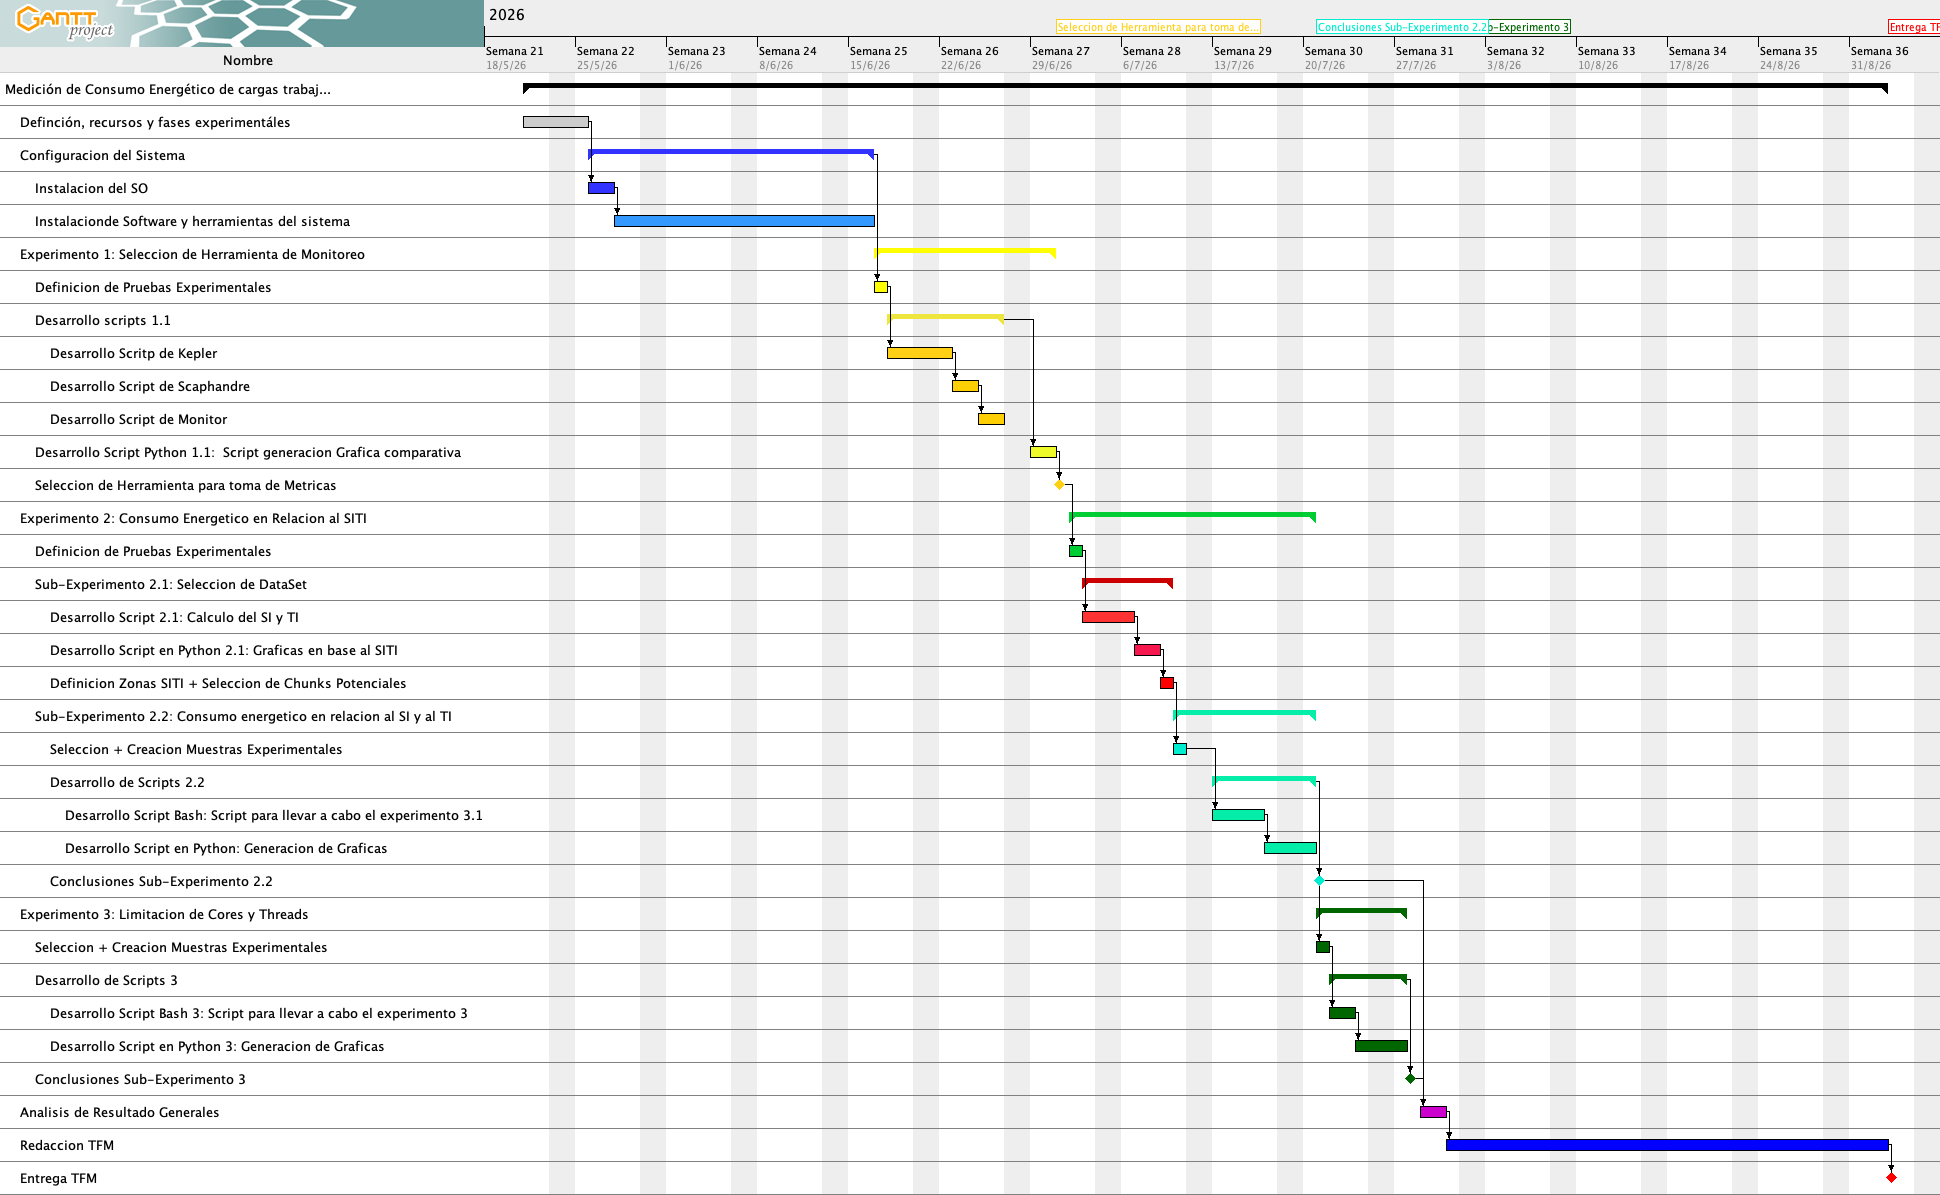
\includegraphics[width=\linewidth]{figs/PlanificacionFinal.png}
     \caption{Ajuste planificacion de desarrollo del Diagrama de Gantt}
     \label{fig:results-gantt-final}
 \end{figure}

 Como resultado del reajuste en tiempo que se muestra en el diagrama de Gantt \ref{fig:results-gantt-final}.
 
 \begin{figure}[ht!]
     \centering
     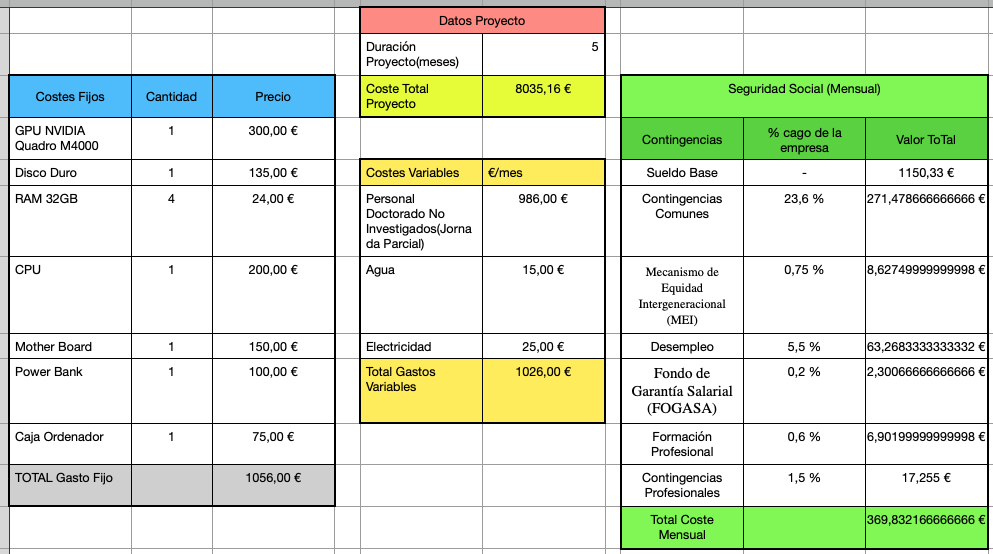
\includegraphics[width=\linewidth]{figs/estimacion-final-coste.png}
     \caption{Header CSV del archivo de datos procesados de Kepler}
     \label{fig:coste-final-spec}
 \end{figure}